\documentclass{beamer}

%\pdfmapfile{+sansmathaccent.map}
%
% Choose how your presentation looks.
%
% For more themes, color themes and font themes, see:
% http://deic.uab.es/~iblanes/beamer_gallery/index_by_theme.html
%
\mode<presentation>
{
  \usetheme{CambridgeUS}      % or try Darmstadt, Madrid, Warsaw, ...
  \usecolortheme{default} % or try albatross, beaver, crane, ...
  \usefonttheme{default}  % or try serif, structurebold, ...
  \setbeamertemplate{navigation symbols}{}
  \setbeamertemplate{caption}[numbered]
} 


\usepackage[T1]{fontenc}

\usepackage[french]{babel}
\usepackage[utf8]{inputenc}
\usepackage{graphicx}
\usepackage{grffile}
\usepackage[absolute,overlay]{textpos}
\usepackage[font={small,it}]{caption}
\captionsetup{position=below}
\usepackage{pgfpages}
%\setbeameroption{show only notes}
\setbeameroption{show notes on second screen=right}
\setbeamertemplate{note page}{\insertnote}

%\insertslideintonotes{0.25}


\newcommand{\backupbegin}{
   \newcounter{finalframe}
   \setcounter{finalframe}{\value{framenumber}}
}
\newcommand{\backupend}{
   \setcounter{framenumber}{\value{finalframe}}
}


\newcommand{\startsection}[1]{
\section{#1}
\begin{frame}{Où en sommes-nous ?}
\tableofcontents[currentsection]
\note{\begin{center}
\insertslideintonotes{0.7}
\end{center}}
\end{frame}
}



\title[Soutenance - Rendu style NOVAT]{Rendu de panorama de montagne dans le style de l'atelier NOVAT}
\subtitle{Superviseurs : Joelle Thollot et Romain Vergne}
\author[J.Granier]{Jonathan Granier}
\date{25 juin 2018}
\institute[Maverick, LJK, INRIA]{MAVERICK (LJK, INRIA)} 


\begin{document}

\begin{frame}
  \titlepage
  \begin{center}
  
\includegraphics[width=0.4\linewidth]{Images/maverick.png}
\end{center}

\note{ Bonjour à tous, je vais vous présenter mon travail effectué dans le cadre de mon stage , fait dans L’équipe Maverick , superviser par ...  \\
\begin{center}
\insertslideintonotes{0.7}
\end{center}
}
\end{frame}


%slide 23 :
%rendu final = ajout ombres portées ? Si oui c'est peut-être plus clair ?
%Tu peux peut-être afficher aussi la carte de hauteur ?

% TODO SCHEMA : slide 36
%1Carte de hauteur original*e* (il y est 2 fois attention)


% TODO LISTE :
% Mesurer le temsp en étant bien lent pour pouvoir etre large. 
% Discours + Note (C'est que la slide apporte + transistion avec la slide suivante)
% Un panorama est une carte sémantiqe avec des degrées de liberté laisser à l'artiste. Il peut modifier 

% Colorisation aquarelle ( faire le dégradé dans la petite case)
% Ajouter du gras sur des mots clef , sur Notre méthode quand on compare (si possible)
 
% Refaire slide exagerated shading. 

% Pas creation panorana arthur . 
% Si le temps (chrono) mettre interview PN , etre plus gentil sur les futurs workks, plus ouvert sur les possibilité

% Faire page de garde

% Section et sous section. 




% Vérifier les fautes d'orthographe : 
% Ombrage on oublie , on parle d'illumination ou de dégradé d'ombre
% 
% Si on a le temps mais ce serai bien de le faire : 
% Ajouter des annexes avec les equations dedans expliquer



% Ce qui a était fait : 
% Ajouter image slide ombrage/ombre portée plus claire puis passer au ombres de PN
% Faire fleche sur le style novat sur ce qu'on veut montrer. 
% Faire la surprise du résultat 
% Faire un cas puis l'autre pour p
% Rajouter transition discontuinuité 
% Montrer l'angle droit quand ça marche pas 
% Schema slide 25
% Adapter avec T
% Virer Euler , osef
% Corriger slide 10 (texte rouge moche)
% Slide Tom : Séparer les couche et faire une somme
% Etat de l'art : prendre autre publie (voir diapo) et prendre image petite fille
% Inverser schéma Vue d'ensemble



%Pas de question réthorique
%Slide -> une utilité 
%Dire les paramètres
%Entourer ce qu'on veut montrer
%Dire que c'est temps réel
%Intranet --> conseil sur les presentation
%Pas de block de texte ni de phrase
%Page de garde logo maverick

%Faire intuitions plus haut niveau
%2 sorte de carte : sémantique , IGN 
%Les panoramas , On peut tricher sur la lumière et la forme 
%Ombrage = Illuminations


%Discours : 
%Plan --> HORIZONTALE
%Soucis --> Limitations
%Le non réalisme de Novat n'est pas un objectif
%Aller retour : Transimition de savoir, Language different
%On est en colaboration avec Arthur Novat.
%Travaux Future : Moins pessimiste , Dire ce qui marche
%Etat de l'art : Transition très violante
%Ambiante occlusion : assombrire les cavités
%Voir : percevoir - perception  
%Rajouter des sousections
%Pourquoi Novat : Porte d'entrée panorama Notre Approche est plus générique
%Les elements de Novat : un peu plus decrires , être plus posé , zoomer sur les ombres à la fin.
%Slide 11 . Montagne cohérente -- Faire des pentes raide ou douces  
%Régle : On s'y perd --> trouver une solution mais réduide la slide
%18 --> On a des probleme de Masquage.
%14  -> image d'internet en petit 
%OM , OP -->fait penser à 2 vecteurs

%Ombre portées : on vire l'abstraction , on dit on tulise un algo standart, le ray marching. (Schema fonction ? )

%Slides 25 : 
%Refaire schema intuitions , faire en sorte qu'il nous suivent pendant l'explication
%Produit plus de variation -> une meilleur perception
%25-2 Horizontal , espace images
%Faire un repere ortho
%25-3 : Pas claire , faire un cas ou q se renverse pas , mettre la formule en bas , rajouter schema intuitions
%Faire THeta = Theta_corrtion par exemple
%Definir Azimute plus clairement
%alpha + theta en italique
%Imager , discontuinuité pas claire
%Spline : smooth step
%Virer P en courbe 
%Dire que T est arbitraire. 


%26 Schema virer lumière , faire plus gros , inverse ombrage lambertione


%Fusion :
%Ref : et al. partout
%Ne pas mettre la courbe --> useless
%faire juste la compairson entre fonction







\section{Contexte}
\subsection*{Résumé}
\begin{frame}

\begin{center}
\only<1>{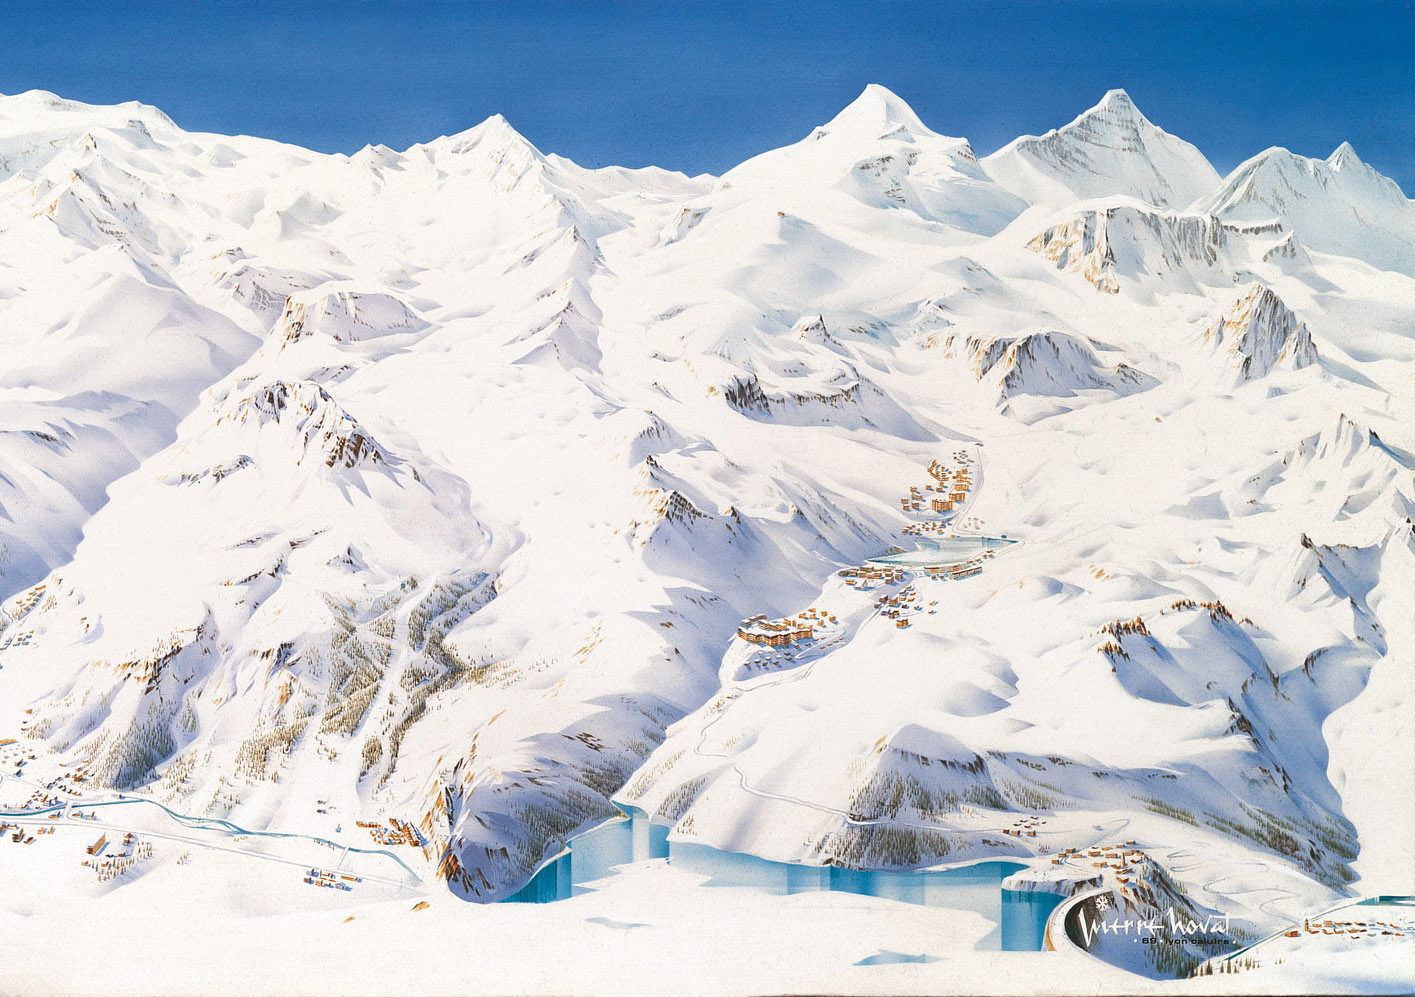
\includegraphics[width=0.9\linewidth]{Images/Val_Isere.jpg}\\}
\only<2>{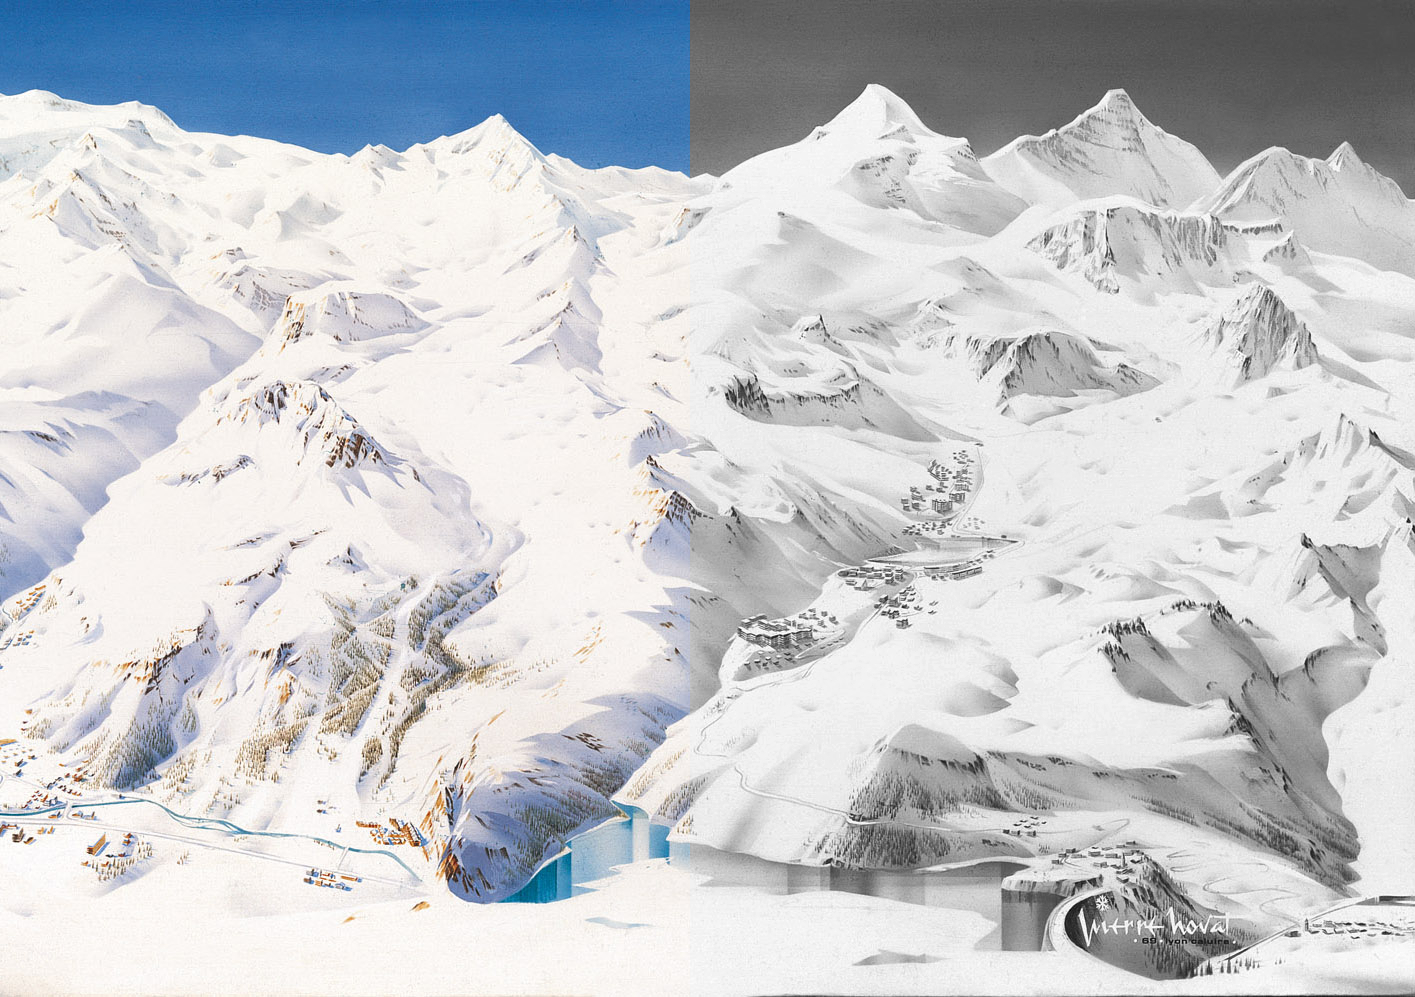
\includegraphics[width=0.9\linewidth]{Images/Val_Isere_gris.jpg}\\}
\textit{Val d’Isere, Tignes, 1967 - Pierre Novat}


\note{\textbf{Mots clés}  : Reproduire panorama - On s'est occupé des ombres \\
\begin{center}
\insertslideintonotes{0.7}
\end{center}
}


\end{center} 

%[Ici on fait un teaser de ce qu'on va faire : Dans ce travail on essaye de reproduire des panoramas plus particulièrement l'ombrage des panorama de Pierre Novat.]
\end{frame}

% Panorama : Représentation visuelle grand angle  
\subsection*{Définition d'un panorama}
\begin{frame}{Définition d'un panorama}
\begin{center}
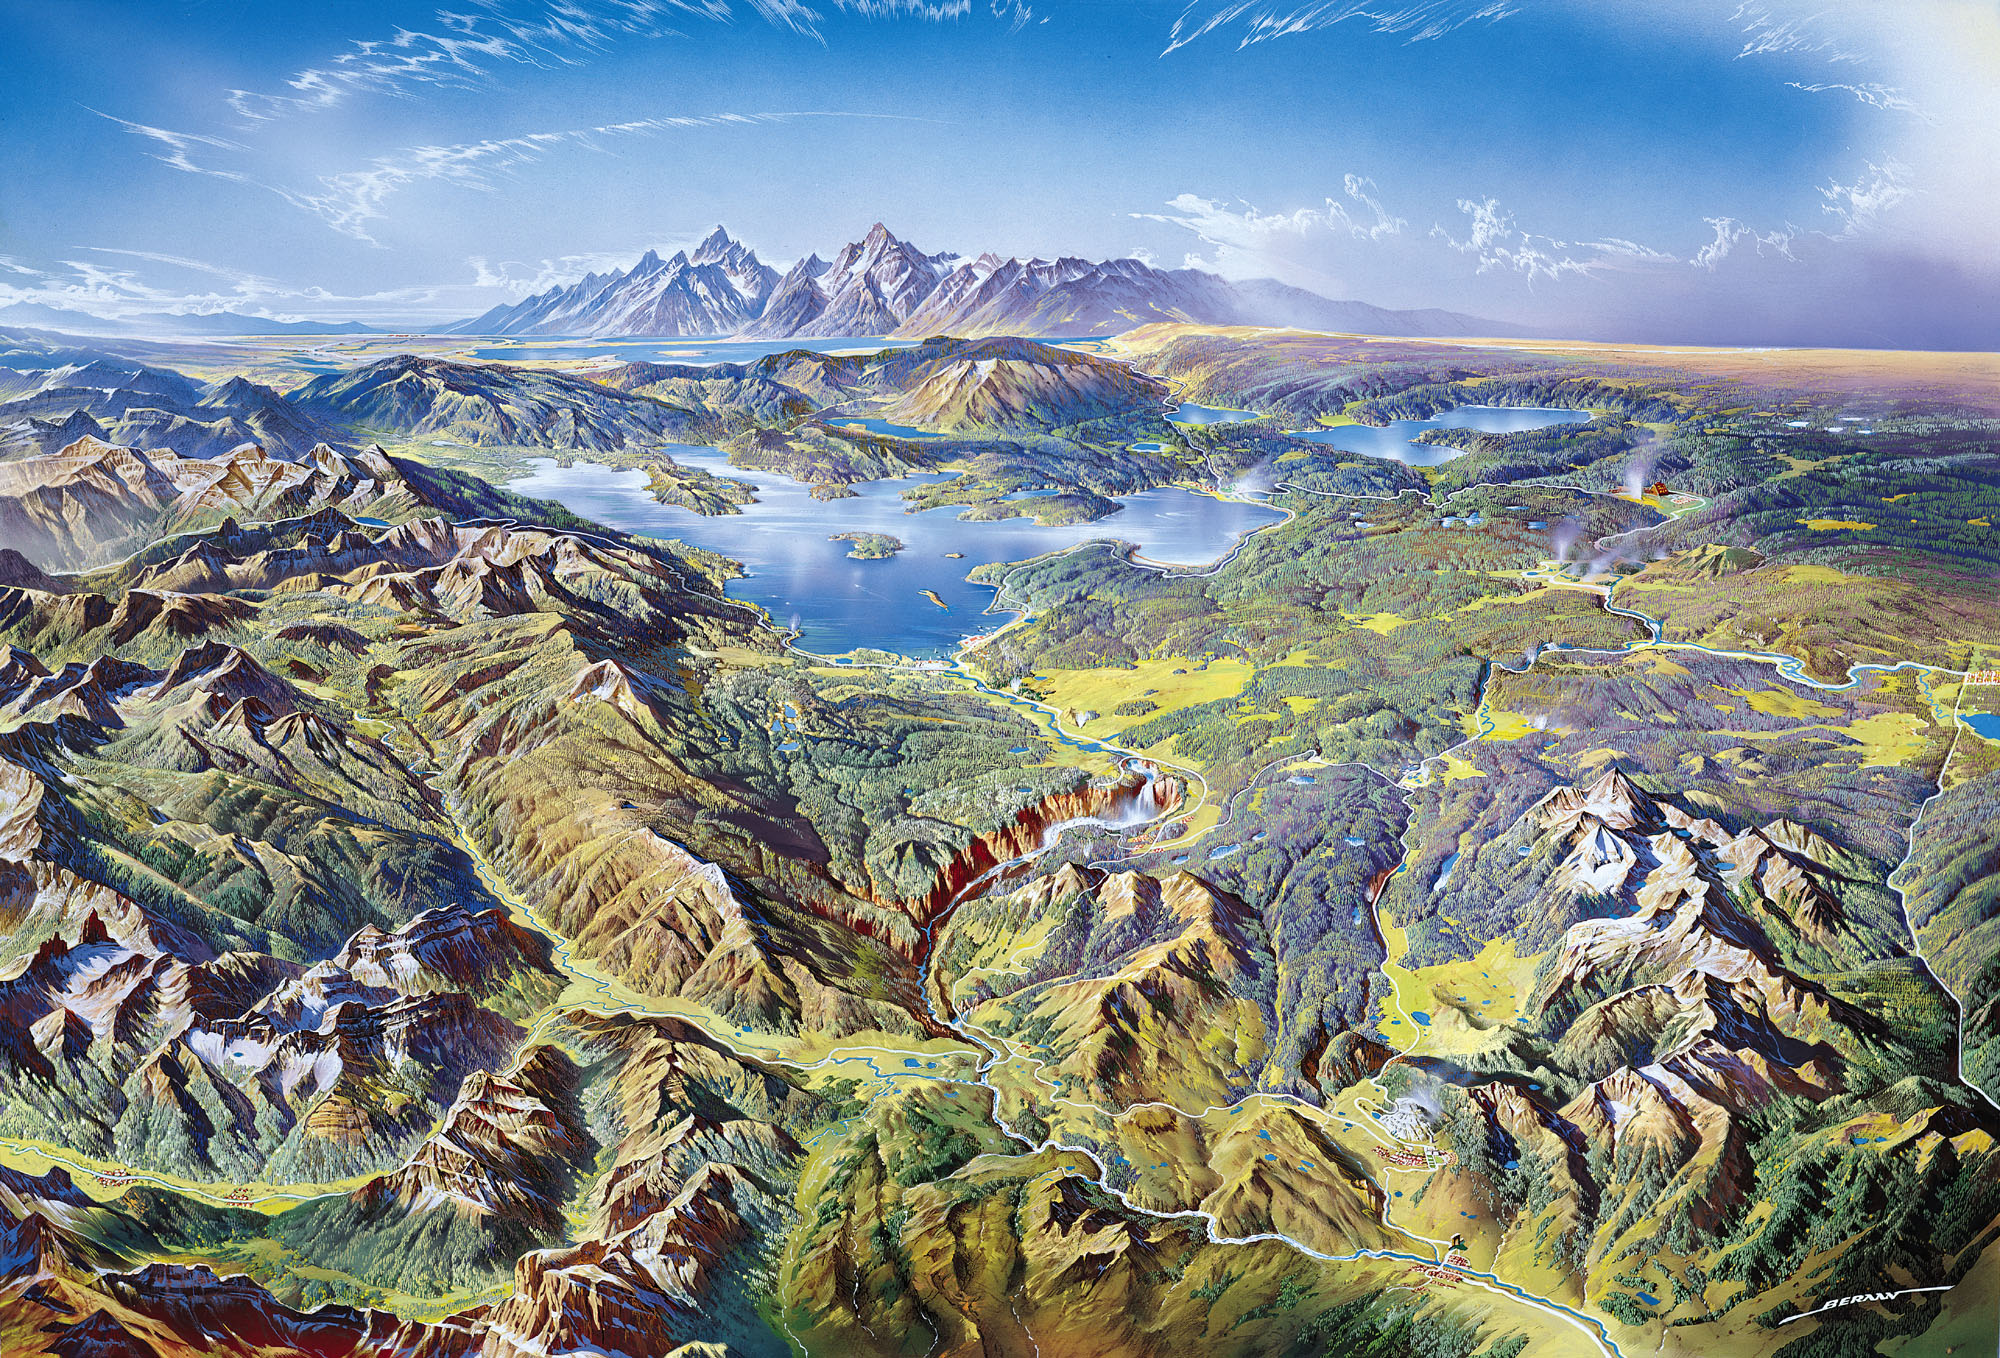
\includegraphics[width=.8\textwidth]{Images/yellowstone_small.jpg}\\
\textit{Parc National du Yellowstone - Heinrich Berann}
\end{center}


\note{
\textbf{Transition} : On va commencer par la définition d'un panorama\\
\textbf{Mots clés}  : Panorama de Heinrich Berann \\
\begin{center}
\insertslideintonotes{0.7}
\end{center}}



\end{frame}
\begin{frame}{Définition d'un panorama}
 
      \begin{itemize}
        \item<1-> Représentation Visuelle grand angle. 
       	\item<2-> Œuvre \textbf{artistique}.
		\item<3-> Carte \textbf{sémantique}.       
      \end{itemize}	
    \begin{center}
    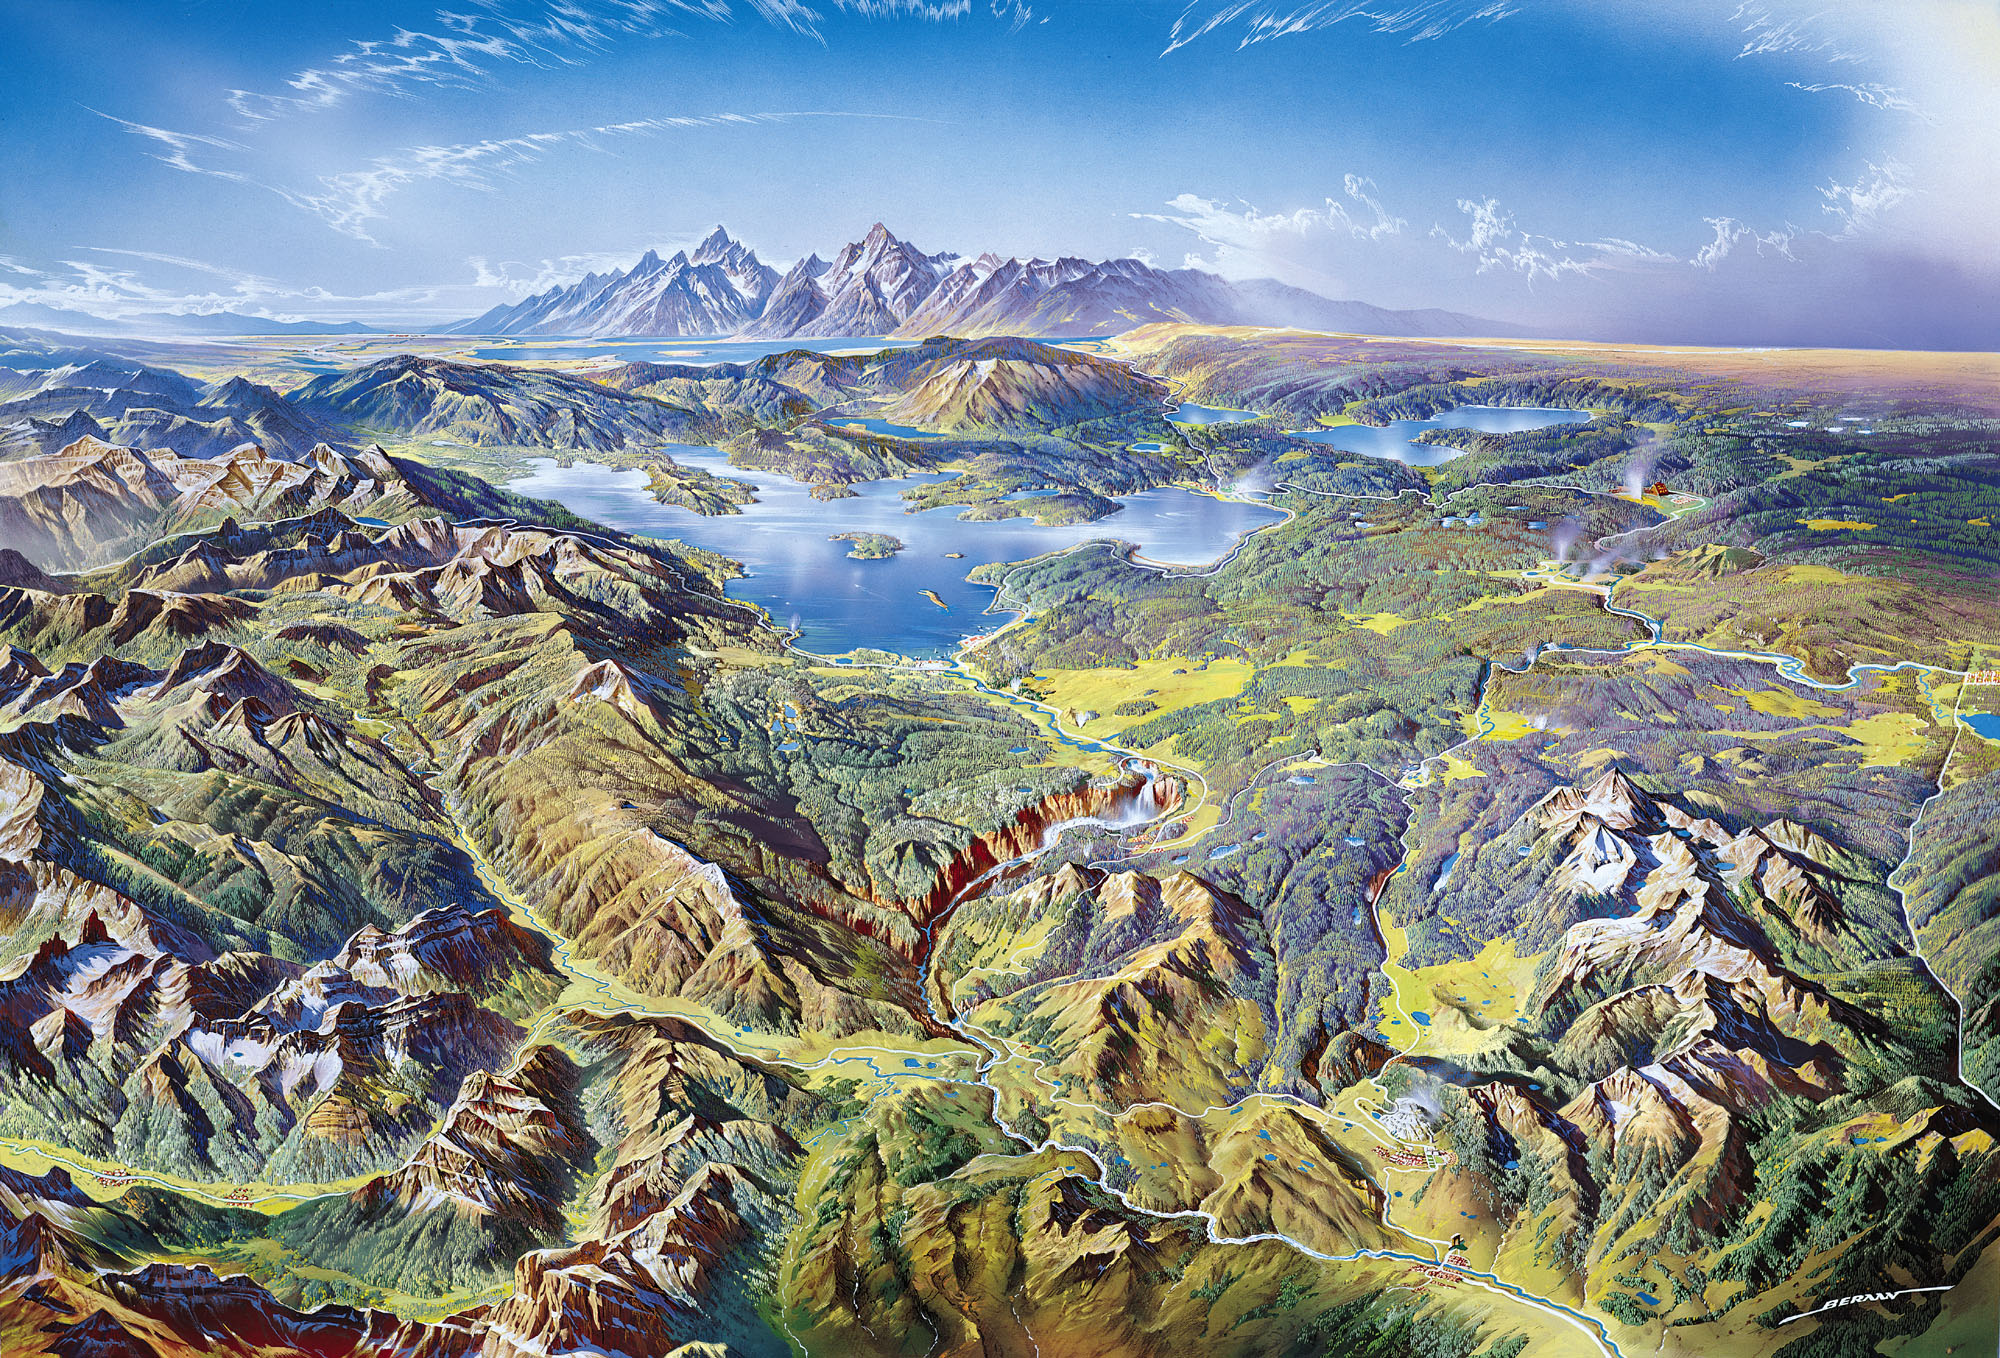
\includegraphics[width=.6\textwidth]{Images/yellowstone_small.jpg}\\
\textit{Parc National du Yellowstone - Heinrich Berann}
    \end{center}
    
\note{
\textbf{Transition} : C'est une représentation grand angle\\
\textbf{Mots clés}  : Tricher sur la forme et la lumière. \\
\begin{center}
\insertslideintonotes{0.7}
\end{center}}




    % Panorama = Carte sémantique 
\end{frame}

\begin{frame}{Définition d'un panorama}
 
    \textbf{Problèmes :}
    \begin{itemize}
    \item Long et compliqué à créer.
    \item Perte de savoir faire. 
    \end{itemize} 
    \visible<2->{
	\textbf{Automatiser} la création de panorama ?
	\begin{itemize}
	\item Stylisation de modèles 3D
	\item Être fidèle à un style artistique. 	
	\end{itemize}
	}
\note{\textbf{Transition} : Seulement la création d'un panorama est un exercice difficile. \\
\textbf{Mots clés}  : Disparition des artistes et sans transmission du savoir \\

\begin{center}
\insertslideintonotes{0.7}
\end{center} }
  
\end{frame}
\subsection*{Le rendu de panorama} 
\begin{frame}{Le rendu de panorama}
Deux publications : [Bratkova et al. 2009],[Brown et al. 2017].
\begin{itemize}
\item Basées sur Heinrich Berann. 
\item Méthode très générale. 
\item Lumière pas traitée.
\end{itemize}	


\begin{center}
    \begin{minipage}[c]{0.45\linewidth}
    \begin{center}
    	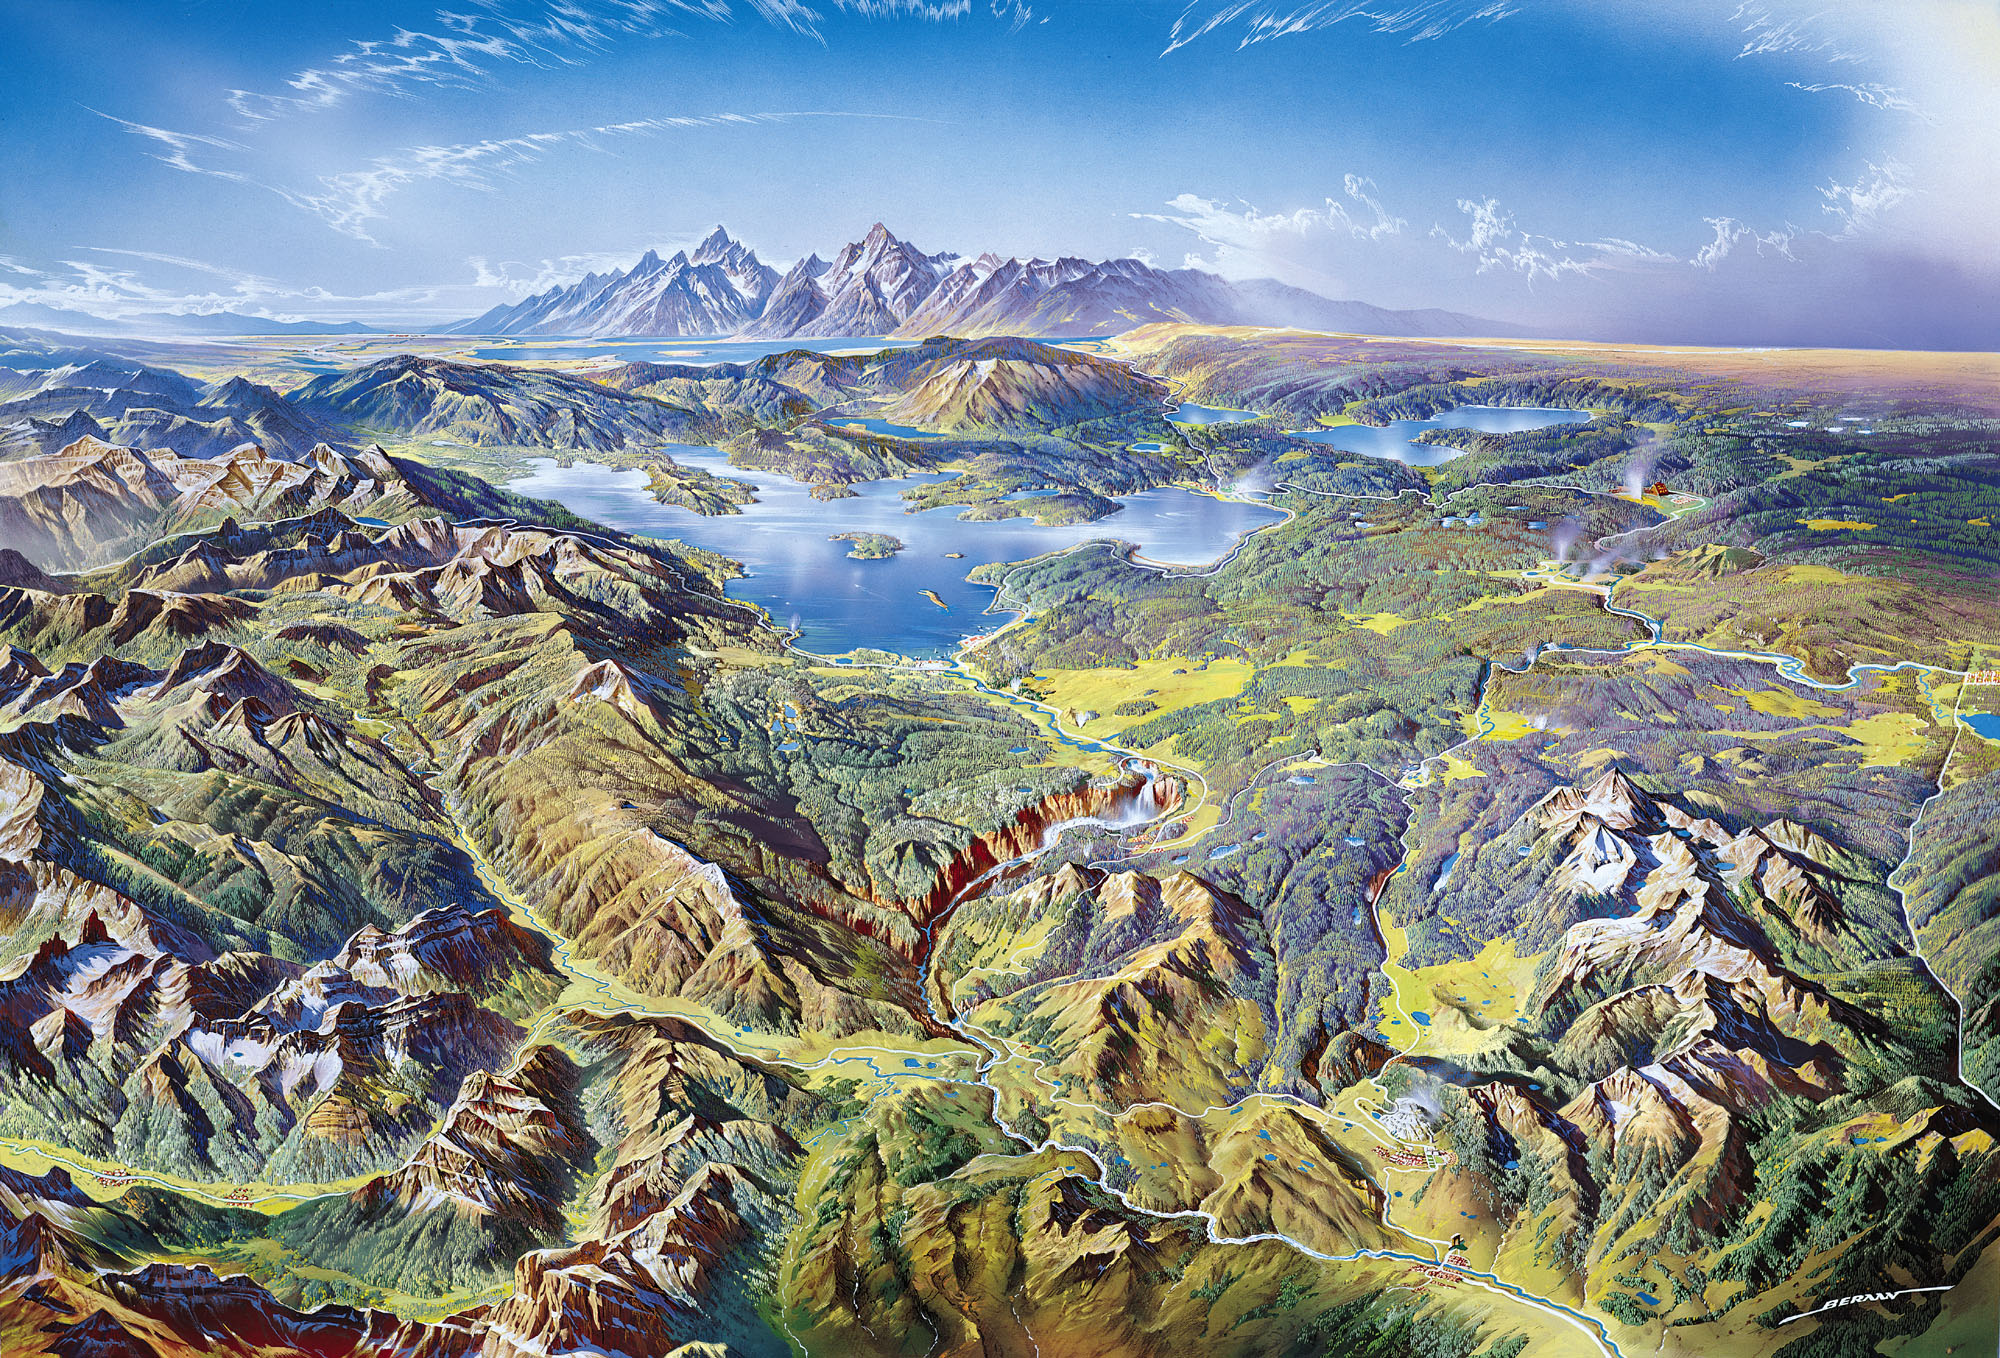
\includegraphics[width=1.0\linewidth]{Images/yellowstone_small.jpg}\\
 		\textit{Parc National du Yellowstone - Heinrich Berann}
    \end{center}
    \end{minipage}
    \hspace{0.2cm}
    \begin{minipage}[c]{0.45\linewidth}
    \begin{center}
    	\includegraphics[width=1.0\linewidth]{Etat_de_lart/resultsYellowstone.png}\\
 		\textit{Rendu du Parc National du Yellowstone - [Brown 2017]}
    \end{center}
    \end{minipage}
\end{center}

\note{
\textbf{Transition} : Dans cette optique, il existe 2 études sur le rendu de panorama. \\
\textbf{Mots clés}: Rendu automatique de panorama - Lumière pas traité. \\

\begin{center}
\insertslideintonotes{0.7}
\end{center}}

\end{frame}

\subsection*{Pierre Novat} 
\begin{frame}{Atelier Novat}
\begin{center}
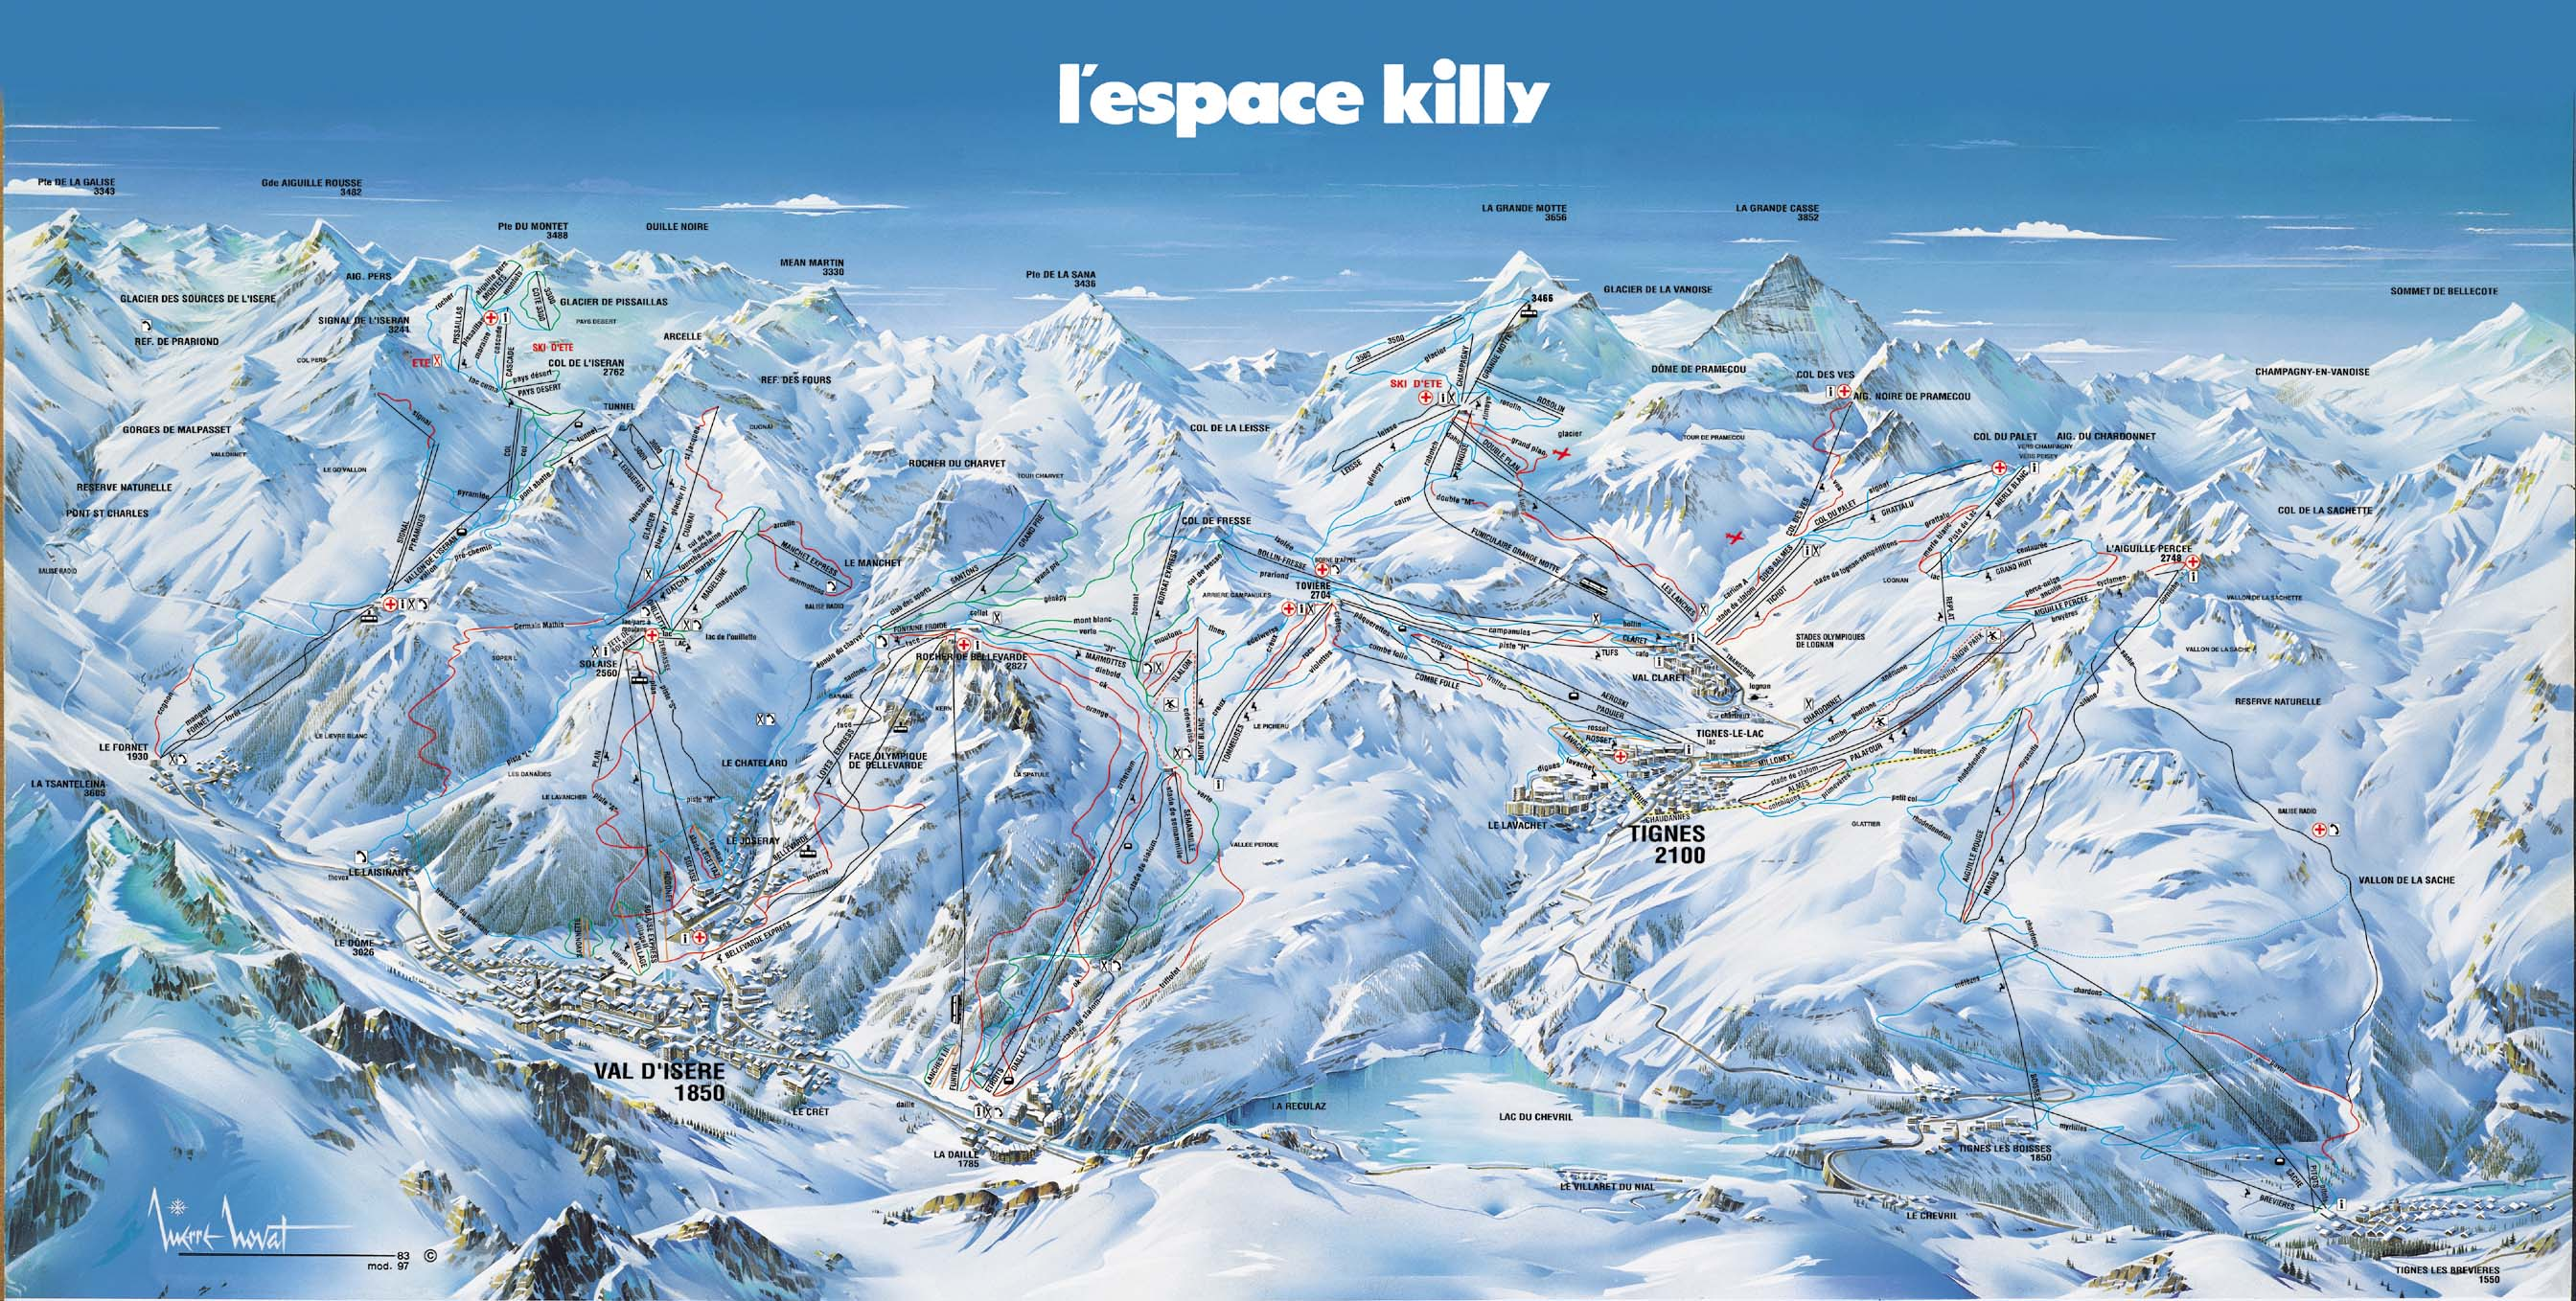
\includegraphics[width=0.9\linewidth]{Images/PN_killy.jpg}\\
\textit{Espace Killy (Val D’Isere, Tignes), 2001 - Pierre Novat}
\end{center}

\note{\textbf{Transition} : De notre côte nous nous sommes penché sur les panoramas de Pierre Novat. \\
\textbf{But}  : Pierre Novat \\
Fondé atelier repris par Arthur Novat \\

\begin{center}
\insertslideintonotes{0.7}
\end{center} }
\end{frame}

\begin{frame}{Projet MECOMO}
MÉmoire, COnnaissance et MOdélisation de la Montagne (2015-2017)\\
Trois axes : 
\begin{itemize}
\item Historique
\item Cognition
\item Informatique
\end{itemize}
Résultats : 
\begin{itemize}
\item Deux articles [Balzarini et al. 2015],[Balzarini et al. 2016].
\item Logiciel prototype sur la déformation de la montagne.
\end{itemize}

\note{
\textbf{Transition} : Dans ce contexte à eu lieu de le projet MECOMO \\
\textbf{Mots clés}  :Projet MECOMO en collaboration avec Arthur Novat. \\
\begin{itemize}
\item Historique : Évolution des stations depuis les 50 dernière années.
\item Cognition : Création et lecture des panoramas.
\item Informatique : Automatisation des panoramas.
\end{itemize}

\begin{center}
\insertslideintonotes{0.7}
\end{center}}

\end{frame}


\begin{frame}{Nos motivations}
Collaboration avec Arthur Novat.
\begin{columns}[t]
  \visible<1->{
  \begin{column}{5cm}
  \begin{exampleblock}{But d'Arthur Novat}
  \begin{itemize}
	\item Transmettre ses connaissances.
	\item Extraire ses algorithmes mentaux de création. 
  \end{itemize}
  \end{exampleblock}
  } 
  \end{column}
  \begin{column}{5cm}
   \visible<2->{
  \begin{exampleblock}{Questions de recherche}
  \begin{itemize}
  \item Comment automatiser la création de panorama ?
  \item Comment lier l'esthétique à la lisibilité ?
  \item Quelle marge de manœuvre pour le designer ? 
  \end{itemize}
  \end{exampleblock}   
   }
  \end{column}
 \end{columns}
\note{
\textbf{Transition} : Nous avons continué cette collaboration pour Automatiser le rendu de panorama\\
\textbf{Mots clés} :Collaboration avec Arthur Novat  \\

\textbf{Temps :} 3'30 min MAX . 	\\
\begin{center}
\insertslideintonotes{0.7}
\end{center}}
\end{frame}

\startsection{Style Novat}
\subsection*{Vue d'ensemble}
\begin{frame}{Style Novat}
\begin{center}
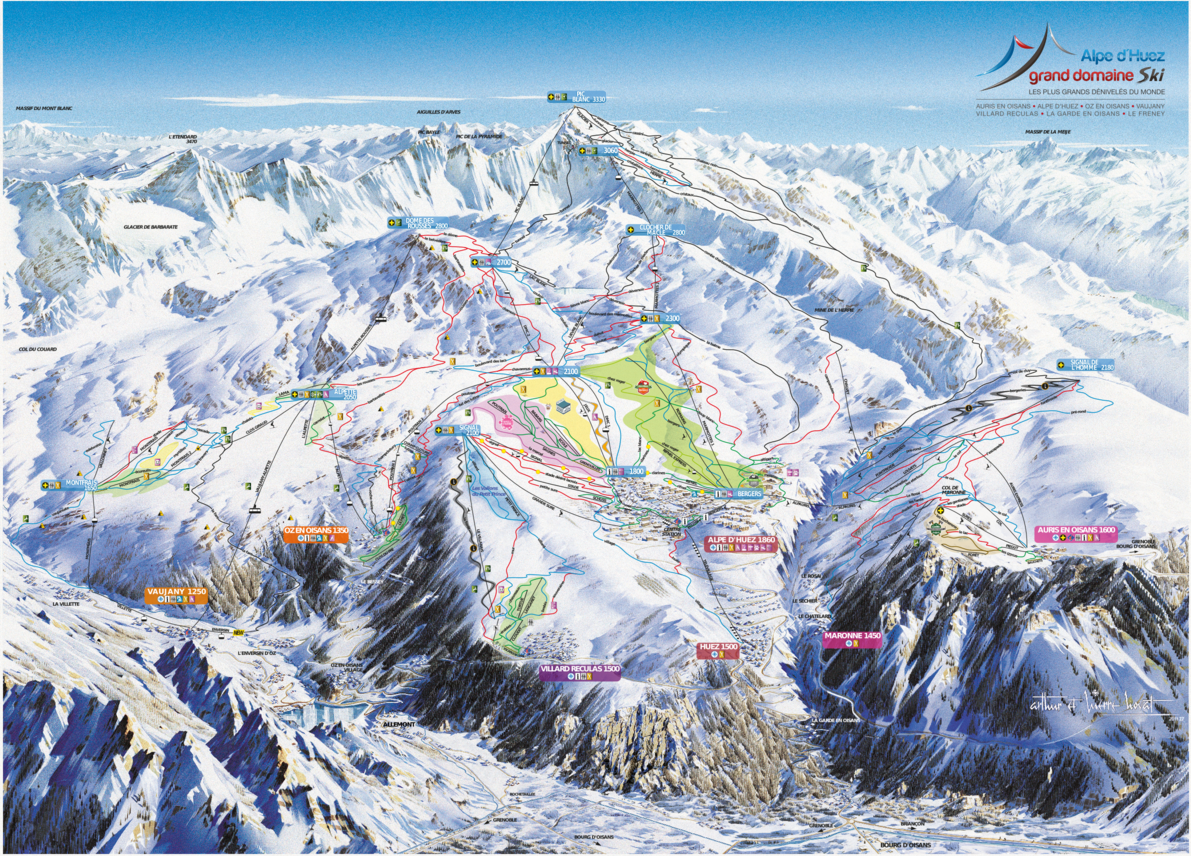
\includegraphics[width=0.8\textwidth]{Images/AlpeHuez_pistes.png}\\
\textit{Plan des pistes de l'Alpe d'Huez - Arthur et Pierre Novat}
\end{center}

\note{\textbf{Transition} :Pour ce faire, nous commençons par une étude du style Novat \\
\textbf{Mots clés} :  Ses panoramas sont complexe et composé de beaucoup d'éléments  \\
\begin{center}
\insertslideintonotes{0.7}
\end{center}}

\end{frame}






\begin{frame}{Les éléments qui composent un panorama}
\begin{center}
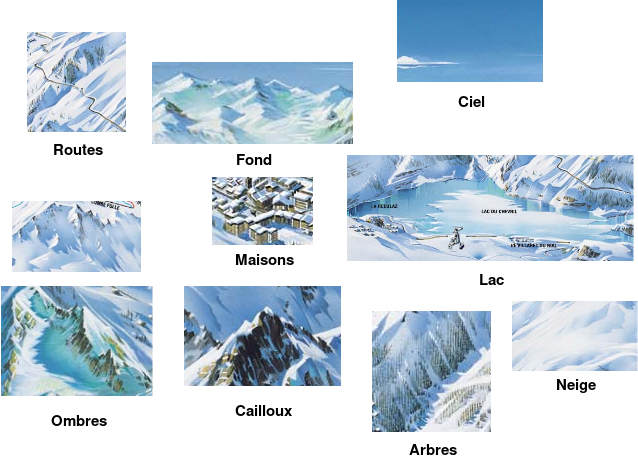
\includegraphics[width=0.8\textwidth]{Images/PN_Elements.png}
\end{center}
\note{\textbf{Mots clés} :  Ombre, élément essentiel pour percevoir la forme - avoir une bonne lisibilité. \\
\textbf{Transition} : C'est pourquoi nous nous sommes plus concentrer dessus.\\
\begin{center}
\insertslideintonotes{0.7}
\end{center}}


\end{frame}


\subsection*{Les ombres de Pierre Novat}
\begin{frame}{Définition des ombres}
    Il y a 2 types d'ombres : 
    \begin{center}
    \begin{minipage}[c]{0.45\linewidth}
    \begin{center}
    	\only<1>{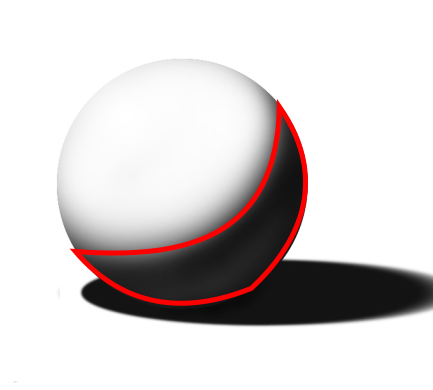
\includegraphics[width=1.0\linewidth]{Schema/ball_illu.png}}
    	\only<2>{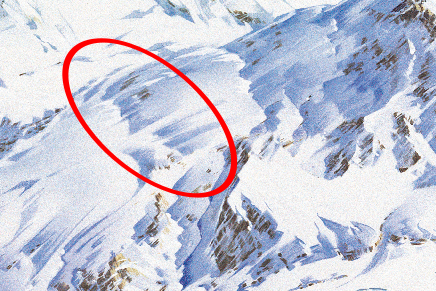
\includegraphics[width=1.0\linewidth]{Images/PN_ombrage_2.png}}\\
 		\textit{Illumination - Dégradé d'ombre}
    \end{center}
    \end{minipage}
    \hspace{0.2cm}
    \begin{minipage}[c]{0.45\linewidth}
    \begin{center}
    	\only<1>{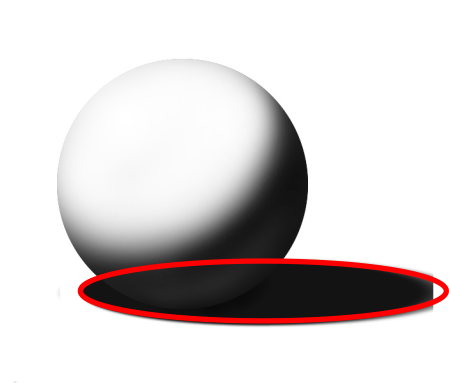
\includegraphics[width=1.0\linewidth]{Schema/ball_shadow.png}}
    	\only<2>{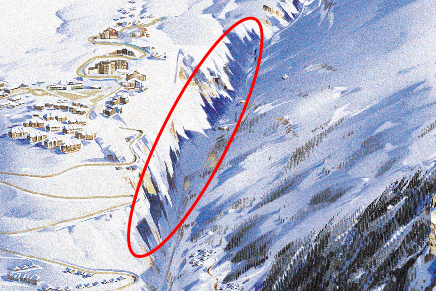
\includegraphics[width=1.0\linewidth]{Images/PN_ombres_portees_2.png}}\\
 		\textit{Ombres portées}
    \end{center}
    \end{minipage}
\end{center}

\note{
\textbf{Transition} : On commence par définir les ombres\\
\textbf{Mots clés} :
\begin{itemize}
\item Illumination : Détermine si une surface fait fasse ou non à la lumière.
\item Ombre portées : Silhouette d'une forme sur une surface.
\end{itemize}

\begin{center}
\insertslideintonotes{0.7}
\end{center} }
\end{frame}


\begin{frame}{Le style des ombres}
	Les caractéristiques des ombres : 
	\begin{itemize}
	\item Fortes et tranchées.
	\item Ombres portées plus effacées que les dégradés d'ombres.
	\item Met en valeur les aspérités.
	\item Cohérence globale, incohérence locale. 
	\end{itemize}
	\begin{center}
	\begin{minipage}[c]{0.45\linewidth}
    \begin{center}
    	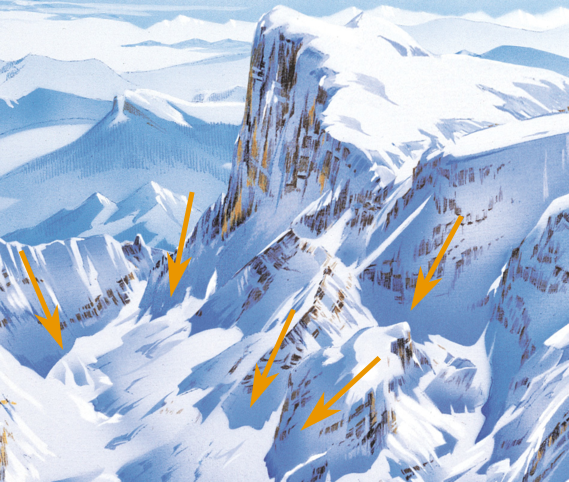
\includegraphics[width=0.9\linewidth]{Images/PN_zoom_ombre_2.png}\\
    \end{center}
    \end{minipage}
    \hspace{0.2cm}
    \begin{minipage}[c]{0.45\linewidth}
    \begin{center}
    	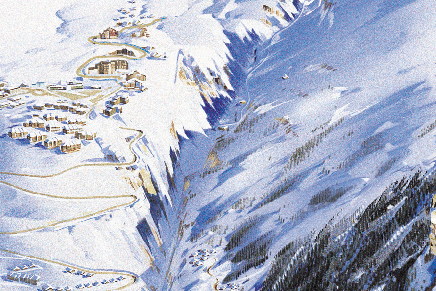
\includegraphics[width=1.0\linewidth]{Images/PN_ombres_portees.png}\\
    \end{center}
    \end{minipage}
	\end{center}
	
	
\note{
\textbf{Transition} : Chez Pierre Novat ces ombres ont plusieurs caractéristiques\\
\textbf{Mots clés} :Meilleur perception du terrain   \\

\textbf{Temps :} 5 min MAX . \\
\begin{center}
\insertslideintonotes{0.7}
\end{center}}
	
	
\end{frame}

\subsection*{Perception de la forme}
\begin{frame}{Perception de la forme}
Direction de lumière
\begin{itemize}
\item Influe la perception [Caniard et al. 2007].
\item Mais est difficile à estimer [Lopez-Moreno et al. 2010]. 
\end{itemize}
\begin{center}
    \begin{minipage}[c]{0.45\linewidth}
    \begin{center}
    	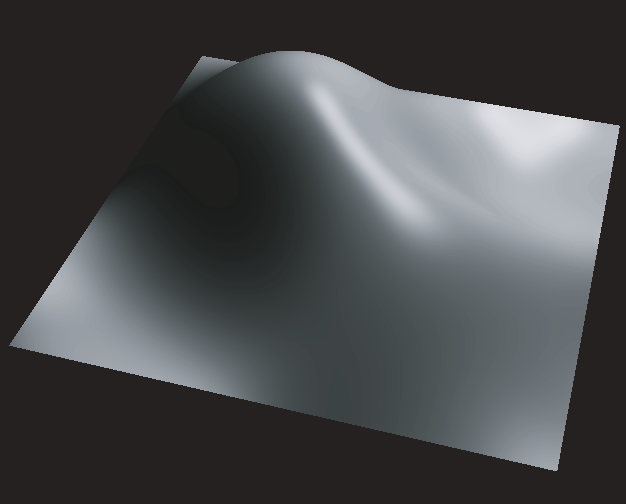
\includegraphics[width=0.8\linewidth]{Etat_de_lart/perception_1.png}
    \end{center}
    \end{minipage}
   % \hspace{0.001cm}
    \begin{minipage}[c]{0.45\linewidth}
    \begin{center}
    	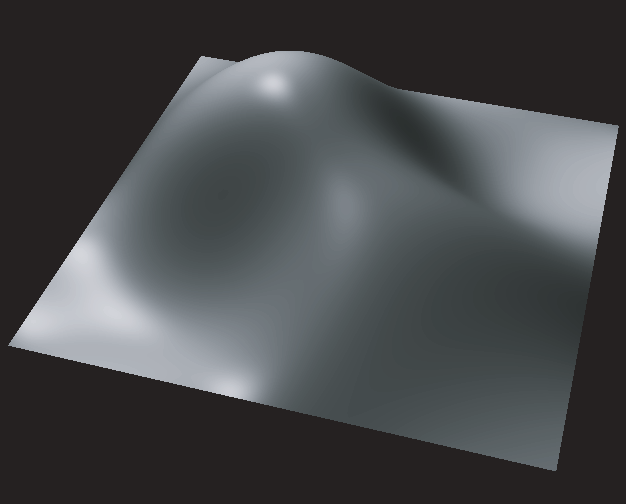
\includegraphics[width=0.8\linewidth]{Etat_de_lart/perception_2.png}
    \end{center}
    \end{minipage}
    ~\\
    \textit{Illumination classique (Phong) mais angle de lumière différent}
	
\end{center}
\note{
\textbf{Transition} : Cette manière de faire rejoints les études faites sur la perception de la forme. 
\textbf{Mots clés}: Notre cerveaux a du mal à estimer. \\
Et donc Pierre Novat utilise ces principes pour dessiner ses ombres \\

\begin{center}
\insertslideintonotes{0.7}
\end{center}}
\end{frame}


\subsection*{Problématique}
\begin{frame}{Problématique}
\visible<1->{
\begin{enumerate}
\item<1-> Faire un rendu temps réel des ombres dans le style des panoramas de l'atelier Novat.
\item<2-> Créer une illumination expressive qui donne à voir toutes les aspérités d'un terrain.
\end{enumerate}
}


\note{
\textbf{Transition} : Ainsi,En s'appuyant sur cette étude précédente, on peut formuler notre problématique \\
\textbf{Mots clés} :
 On va donc s'intéresser à l'illumination dans la cartographie et l'informatique graphique.  \\
\textbf{Temps :} 5'30 min MAX . \\
\begin{center}
\insertslideintonotes{0.7}
\end{center} }
\end{frame}

\startsection{État de l'art}
\subsection*{L'illumination en cartographie}
\begin{frame}{L'illumination en cartographie}
%\begin{center}
\begin{minipage}[b]{0.7\textwidth}
Les conseils de Tom Paterson : 
\visible<2->{
\begin{itemize}
\item<2-> Correction de la lumière localement.
\item<3-> Plusieurs couches d'illumination.
\end{itemize}	
\begin{center}
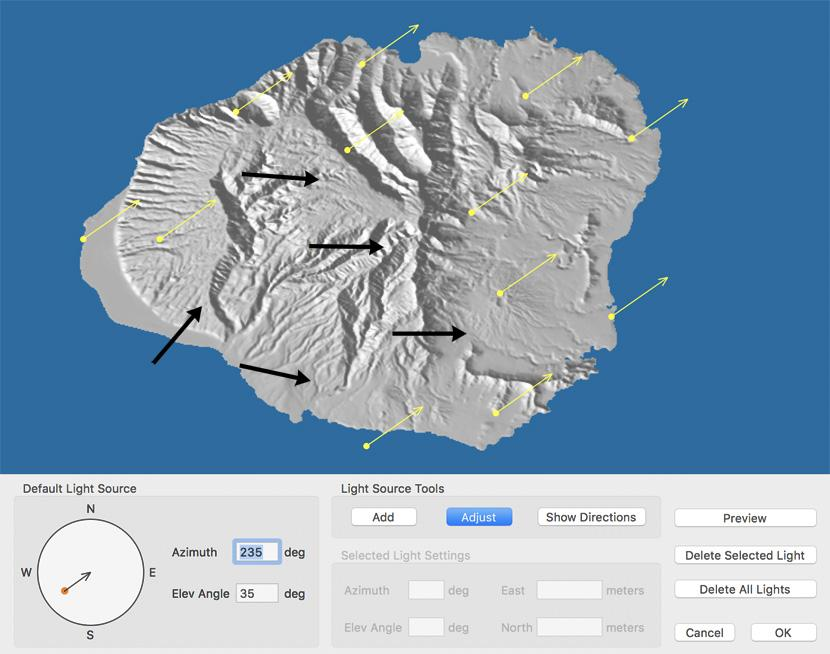
\includegraphics[width=0.7\linewidth]{Etat_de_lart/multiple_light.jpeg}
\end{center}
}
\end{minipage}
\hspace{0.001cm}
\visible<3->{
\begin{minipage}[t]{0.2\textwidth}	
\begin{center}
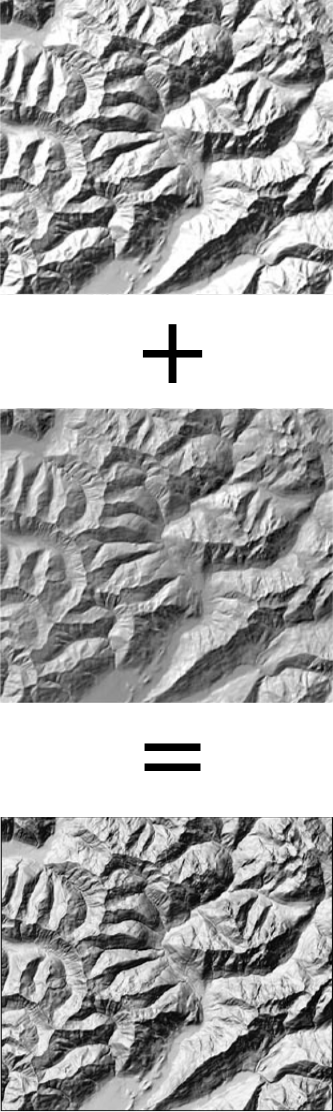
\includegraphics[width=0.9\textwidth]{Etat_de_lart/tom_fusion.png}
\end{center}
\end{minipage}}

\note{\textbf{Mots clés} :Du coté de la cartographie\\
 Tom paterson : Grand cartographe \\
Sur ordinateur, il conseil de faire plusieur couche d'illumination puis de les fusionner , afin de faire apparaitre des éléments qui serai masqué dans une couche et visible dans l'autre  \\

\begin{center}
\insertslideintonotes{0.7}
\end{center} }

\end{frame}
\subsection*{L'illumination exagérée en informatique graphique}
\begin{frame}{L'exagération des ombres en informatique graphique}
     \visible<1->{ 
      \begin{itemize}
        \item<1-> Occlusion ambiante [Pharr et al. 2004].
        \item<2-> 3D Unsharp Masking - Cornsweet Illusion [Ritschel et al. 2008].
        \item<3-> Radiance scaling [Vergne et al. 2010]. 
      \end{itemize}	
    }
    \begin{center}
    	\only<1>{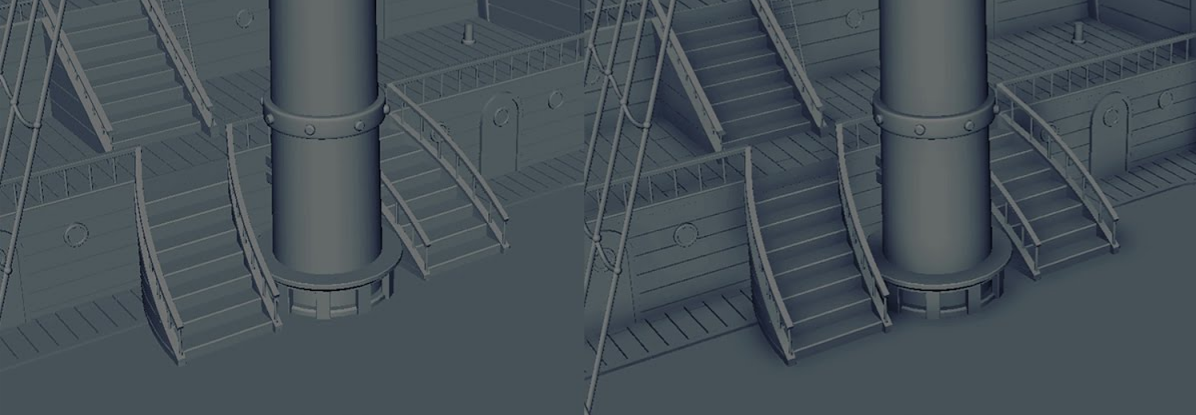
\includegraphics[width=0.8\linewidth]{Etat_de_lart/Ambiante_occlusion.png}~\\
    		\textit{Illumination classique (Gauche) - Occlusion ambiante (Droite)}}
    	\only<2>{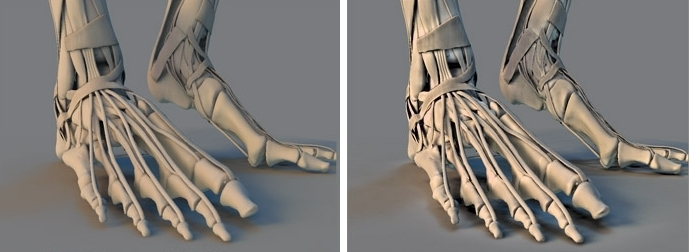
\includegraphics[width=0.8\linewidth]{Etat_de_lart/cornswett.png}~\\
    		\textit{Illumination classique (Gauche) - 3D Unsharp Masking (Droite)}}
    	\only<3>{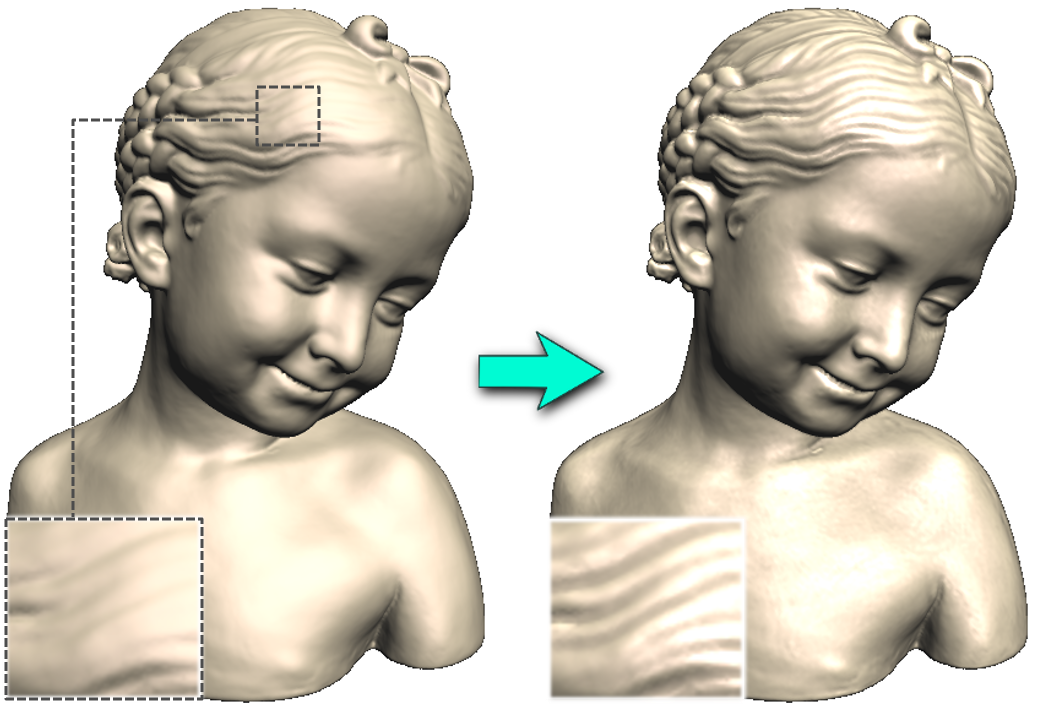
\includegraphics[width=0.5\linewidth]{Etat_de_lart/radiance_scaling.png}~\\
    		\textit{Illumination classique (Gauche) - Radiance Scaling (Droite)}}
	\end{center}
	
	

\note{
\textbf{Transition} : Ensuite du coté de l'informatique graphique , il existe plusieurs méthode d'illumination pour mettre en valeur la forme. \\
\textbf{Mots clés}
\begin{itemize}
\item Ambiante occlusion : Faire ressortir les cavités.
\item 3D unsharp Masking : Faire un filtre en utilisant l'illusion de Cornsweet.
\item Radiance scaling : Moduler l'illumination grâce à la courbure
\end{itemize}
Technique non applicable sur un terrain. \\
\begin{center}
\insertslideintonotes{0.7}
\end{center} }	
	
\end{frame}


\subsection*{Une illumination type carte}
\begin{frame}{Exagerated shading [Rusinkiewicz et al. 2006]}
\begin{itemize}
\item Proche d'une illumination de carte vue de dessus.
\item Lumière rasante.
\item Multi-échelle.
\item Modification de l'élévation de la lumière sur chaque échelle.
\end{itemize}	
\begin{center}
    \begin{minipage}[c]{0.45\linewidth}
    \begin{center}
    	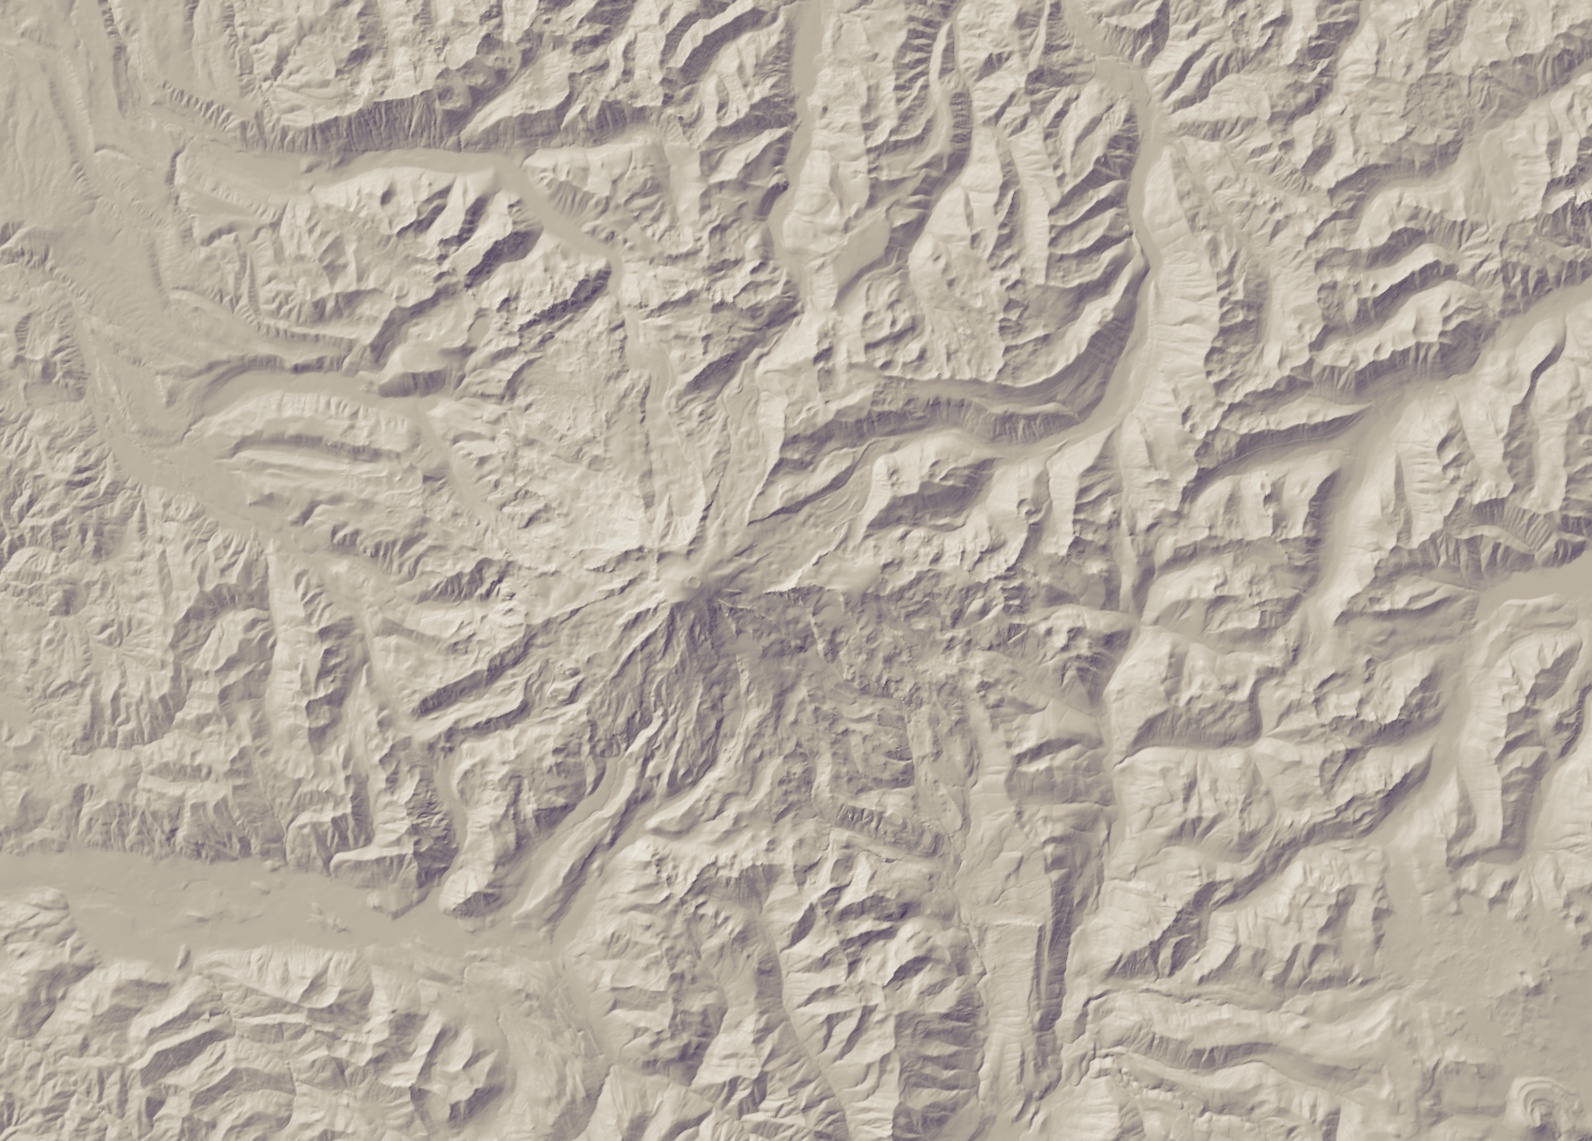
\includegraphics[width=1.0\linewidth]{Etat_de_lart/terrain_diffuse.jpg}\\
    	\textit{Illumination classique}
    \end{center}
    \end{minipage}
   % \hspace{0.001cm}
    \begin{minipage}[c]{0.45\linewidth}
    \begin{center}
    	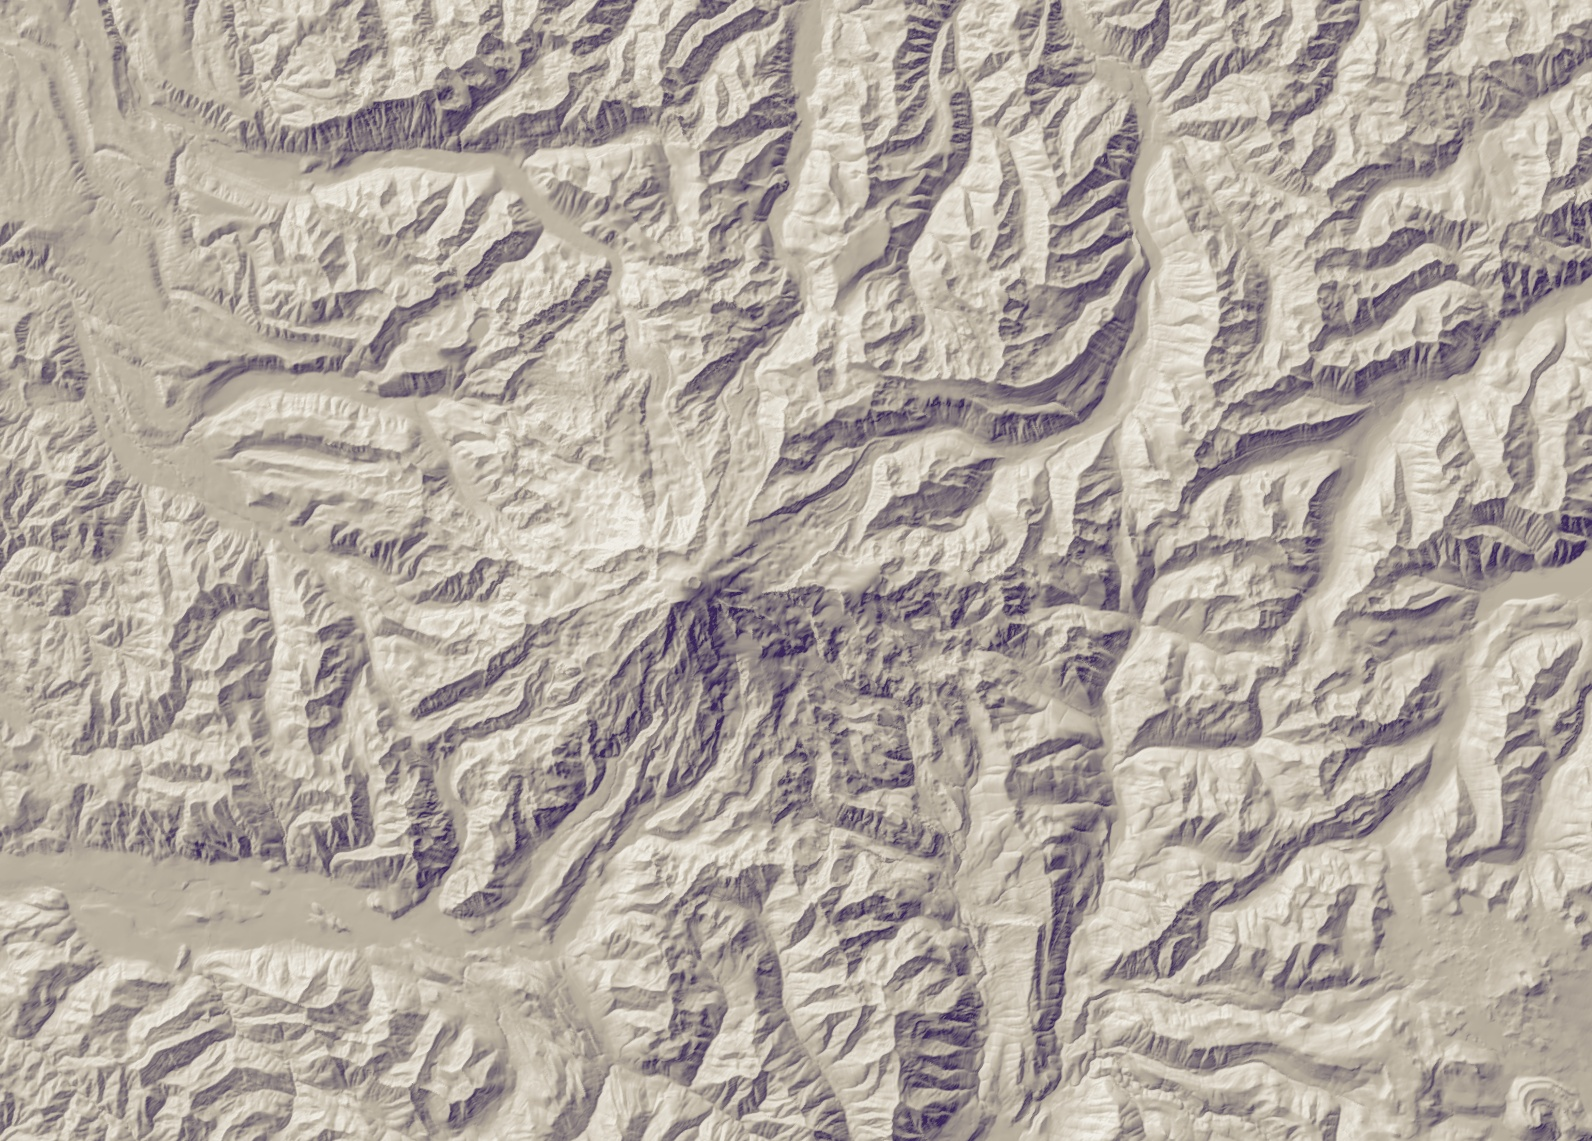
\includegraphics[width=1.0\linewidth]{Etat_de_lart/terrain_exag.jpg}\\
    	\textit{Exagerated shading}
    \end{center}
    \end{minipage}
   
\end{center}


\note{
\textbf{Transition} : En revanche  \\
\textbf{Mots clés} : 
Idée principal : une lumière rasante permet de mieux voir les aspérités.\\
Défaut : Donne une effet bas relief. \\
Cependant on s'inspire de leur méthode. \\
\textbf{Temps :} 8'00 min MAX .\\
\begin{center}
\insertslideintonotes{0.7}
\end{center}} 	

\end{frame}

\startsection{Contribution}
\subsection*{Vue d'ensemble}
\begin{frame}{Vue d'ensemble}
Règles :
\visible<2->{ 
\begin{enumerate}
\item<2-> Cohérence globale.
\item<3-> Direction de la lumière ajustée localement.
\item<4-> Plusieurs niveaux d'illumination. 
\item<5-> Ombres portées moins intenses.
\end{enumerate}
}

\note{\textbf{Mots clés} : On cherche à Améliorer la perception du terrain \\
\begin{center}
\insertslideintonotes{0.7}
\end{center}}	
	


\end{frame}


\begin{frame}{Vue d'ensemble}
\begin{center} 
        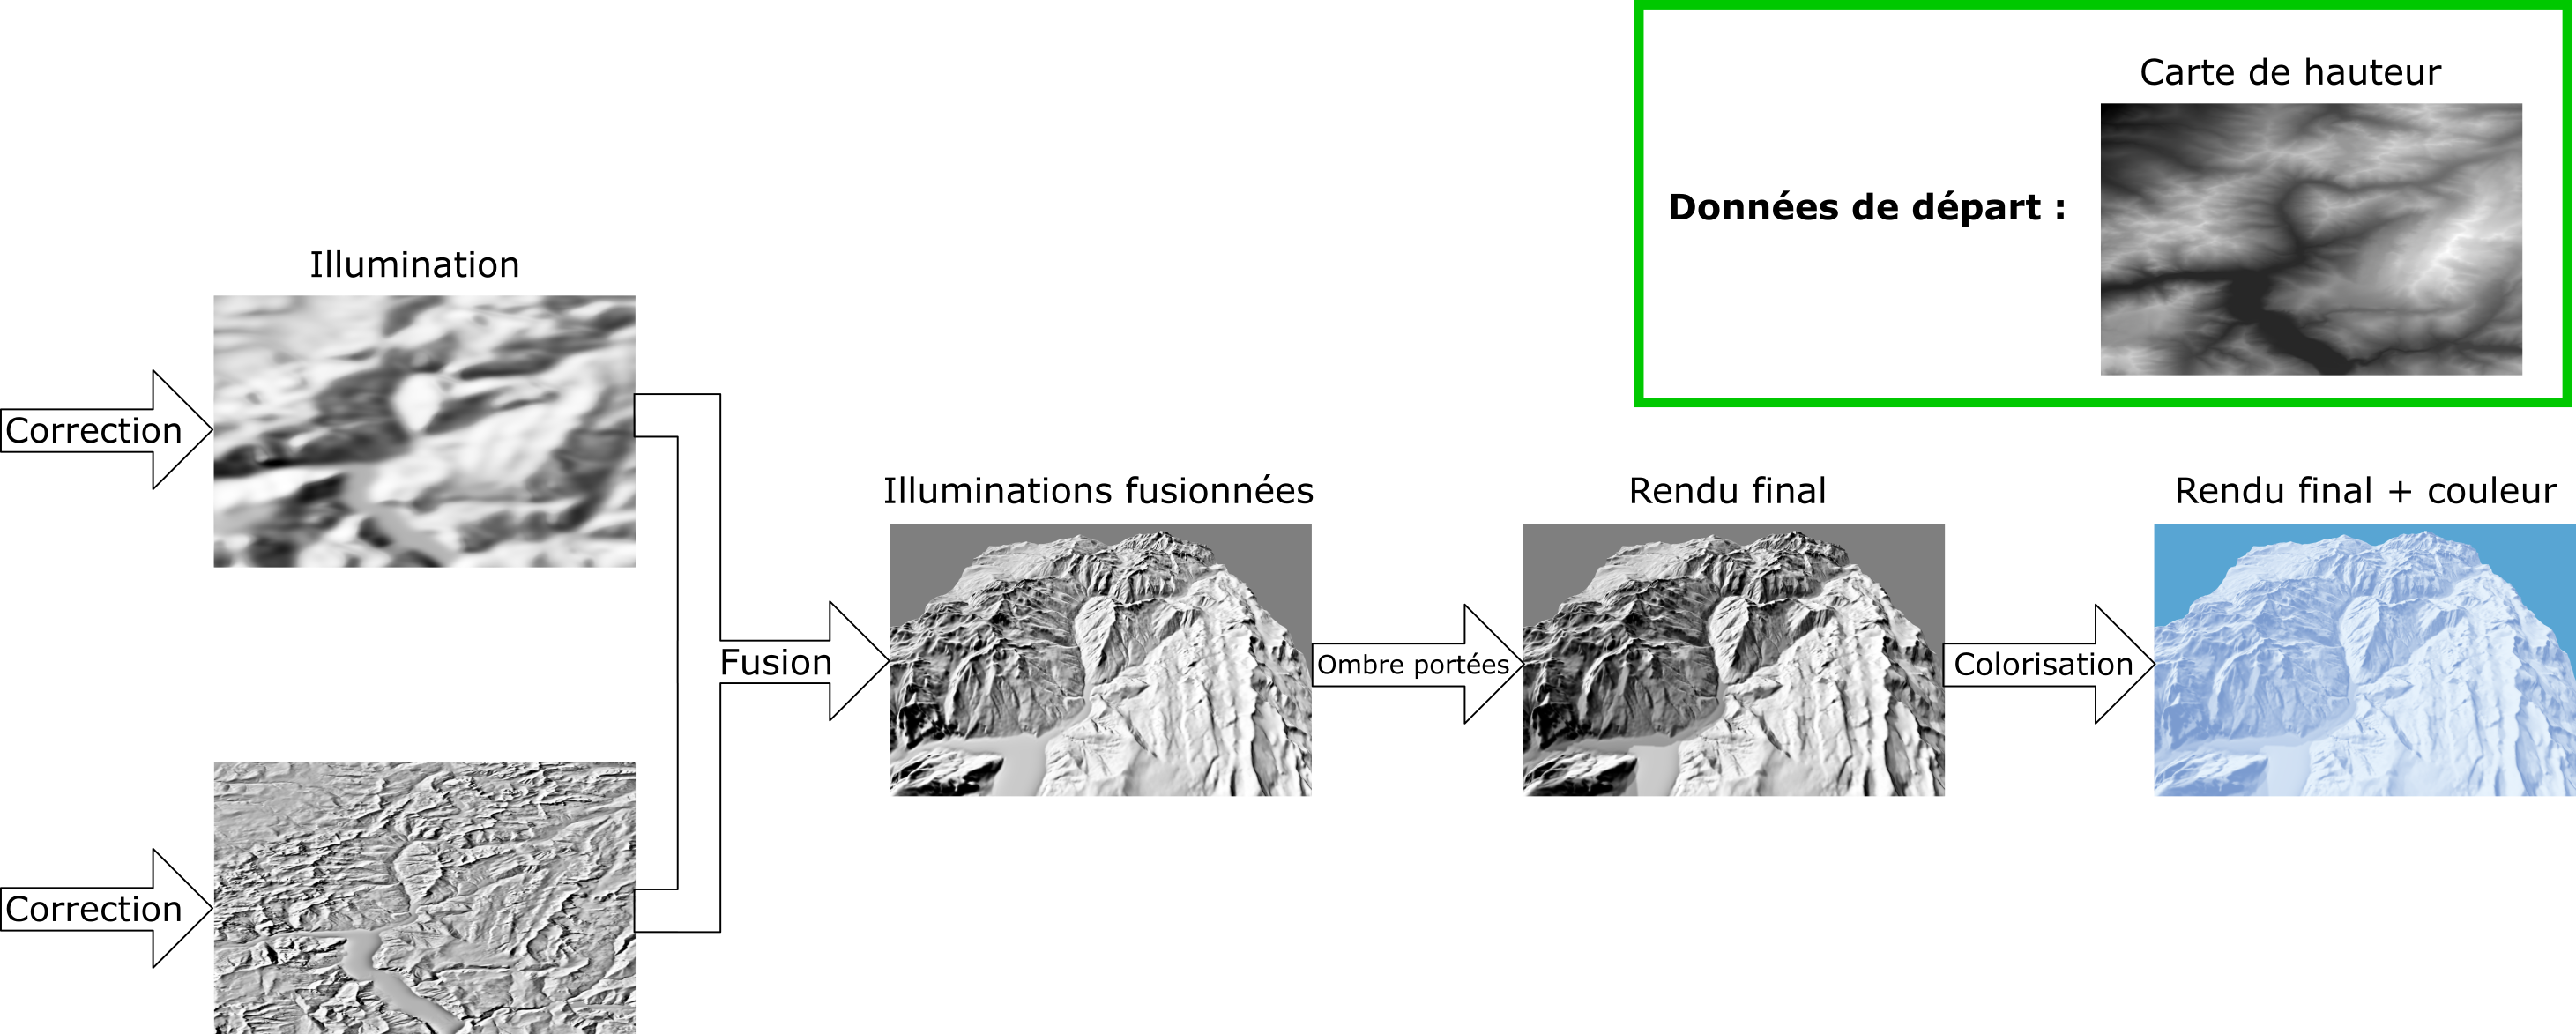
\includegraphics[width=1.0\linewidth]{Schema/pyramide_Laplace_image_resume.png}
\end{center}
\note{
\textbf{Transition} : Ainsi voici notre solution.\\
\textbf{Mots clés} : Correction local de la lumière 
Multi échelle  \\
\begin{center}
\insertslideintonotes{0.7}
\end{center}}	
	

\end{frame}


\subsection*{Orientation locale de la lumière sur une échelle}
\begin{frame}{Orientation locale de la lumière sur une échelle}

\begin{center} 
        \only<1>{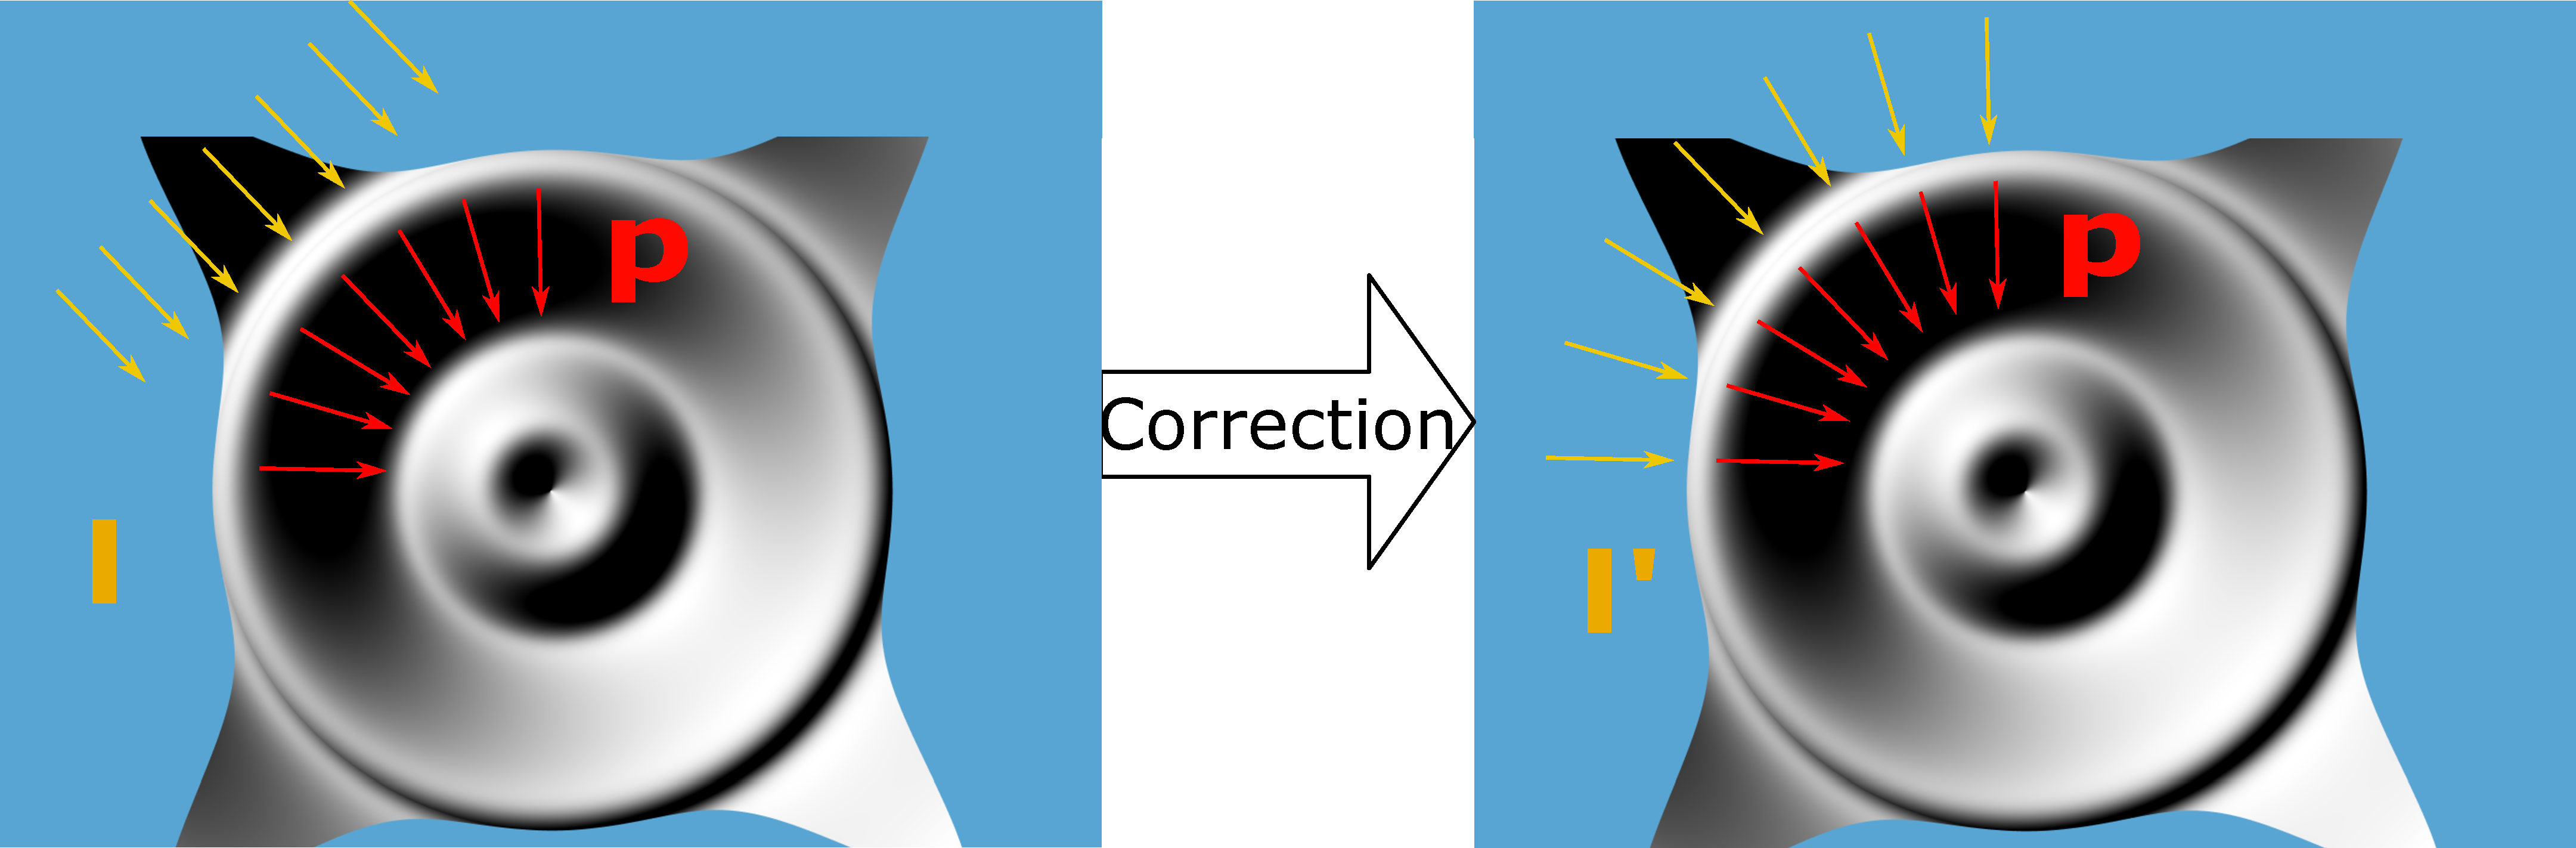
\includegraphics[width=1.0\linewidth]{Schema/correction_light_v4.pdf}}
 		\only<2>{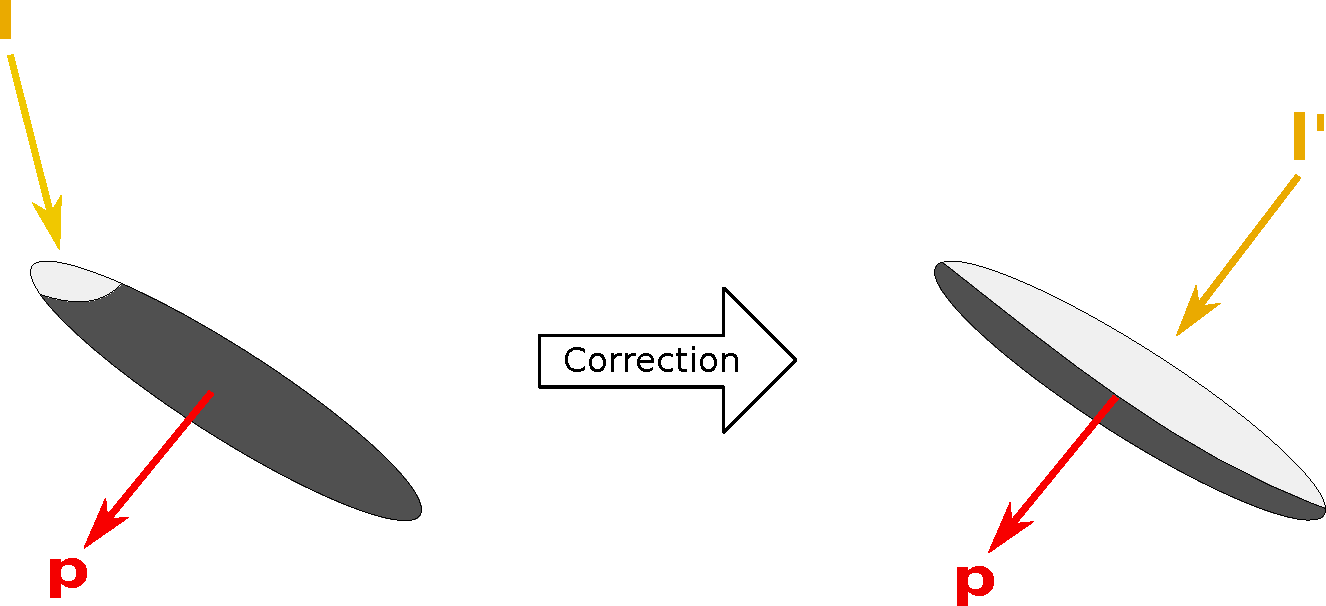
\includegraphics[width=1.0\linewidth]{Schema/correction_light.pdf}}

\end{center}


\note{
\textbf{Transition} : Dans un premier on s'occupe de la correction local sur une échelle.\\
\textbf{Mots clés} :Intuitions  \\
Pas élévation , uniquement de l'azimute.  \\
Correction sur le plan horizontal.\\
Aligner l'azimut - pente LOCALEMENT.  \\

\begin{center}
\insertslideintonotes{0.7}
\end{center}}	
	



\end{frame}

\begin{frame}{Calcul $\theta_{corr}$ : Deux cas possibles}
\begin{center}
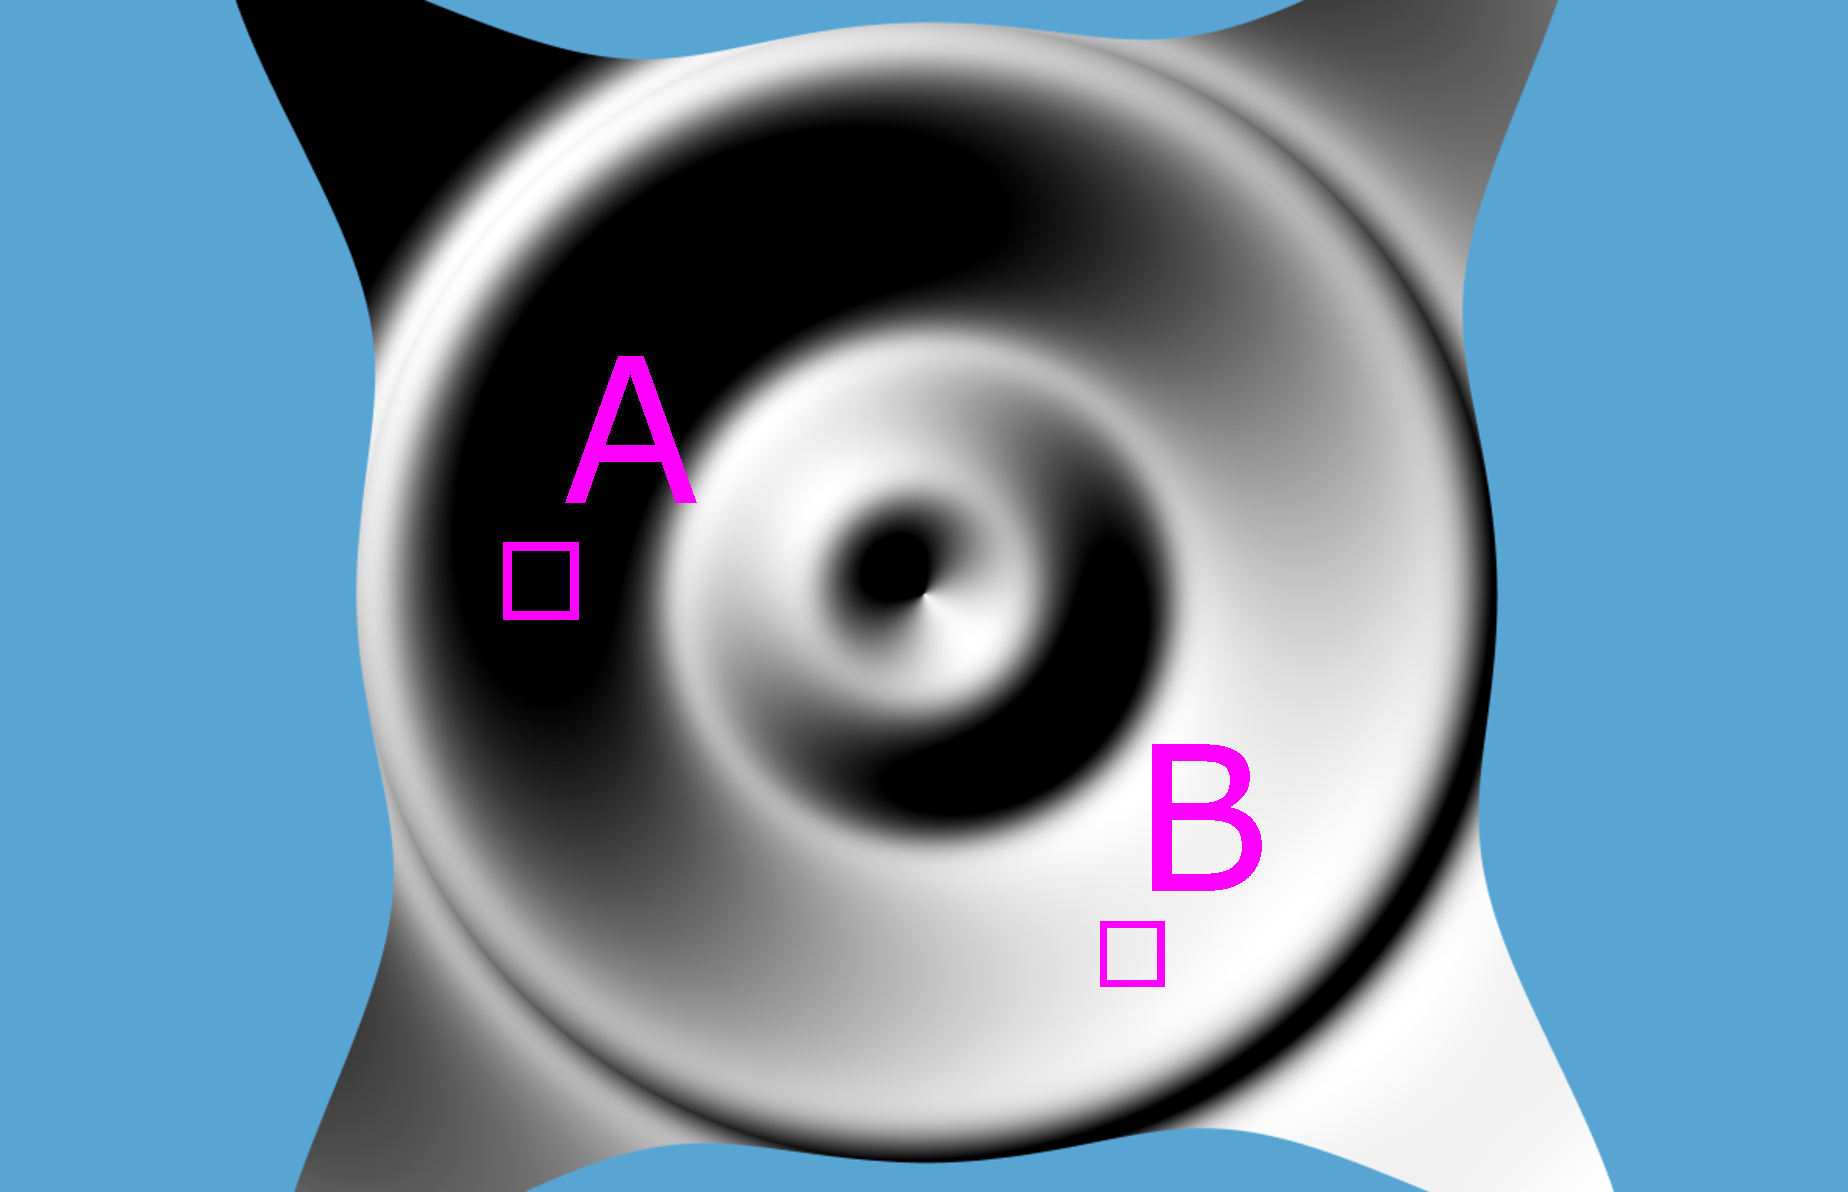
\includegraphics[width=0.8\linewidth]{Schema/orientationTheta_Image_1.pdf}
\end{center}

\note{
\textbf{Transition} : Il y a deux cas possible .\\
\textbf{Mots clés} : A et B deux points \\

\begin{center}
\insertslideintonotes{0.7}
\end{center}}	
	


\end{frame}

\begin{frame}{Calcul $\theta_{corr}$ : Cas A}
\begin{center}
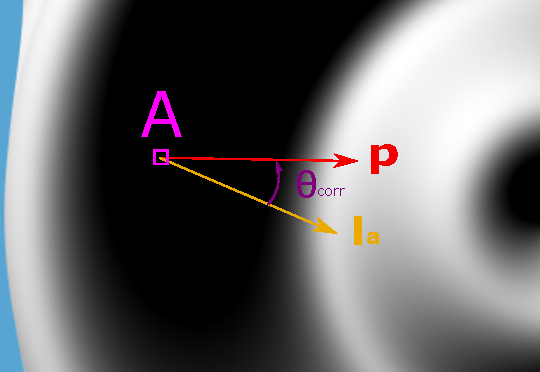
\includegraphics[width=0.8\linewidth]{Schema/orientationTheta_Image_2.pdf}\\
\textit{Cas où $\vec{l_a}\cdot \vec{p} \geq 0$}
\end{center}

\note{
\textbf{Transition} :  Le cas A .\\
\textbf{Mots clés} :Pente même direction que  la lumière \\

\begin{center}
\insertslideintonotes{0.7}
\end{center}}	
	


\end{frame}

\begin{frame}{Calcul $\theta_{corr}$ : Cas B}
\begin{center}
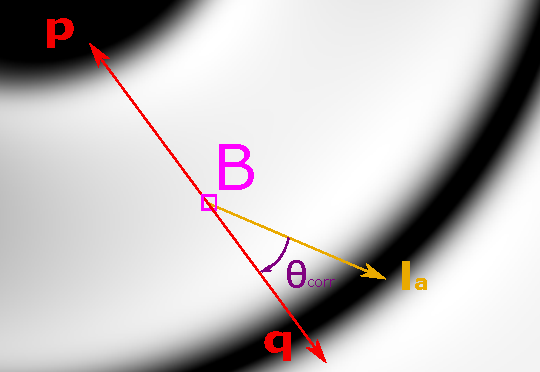
\includegraphics[width=0.8\linewidth]{Schema/orientationTheta_Image_3.pdf}\\
\textit{Cas où $\vec{l_a}\cdot \vec{p} \leq 0$}
\end{center}
\note{
\textbf{Transition} :  Cependant dans le cas B .\\
\textbf{Mots clés} :Pente  direction opposé à la lumière \\
Q , pente opposé \\

\begin{center}
\insertslideintonotes{0.7}
\end{center}}	
	


\end{frame}

\begin{frame}{Correction simple}

\begin{center} 
        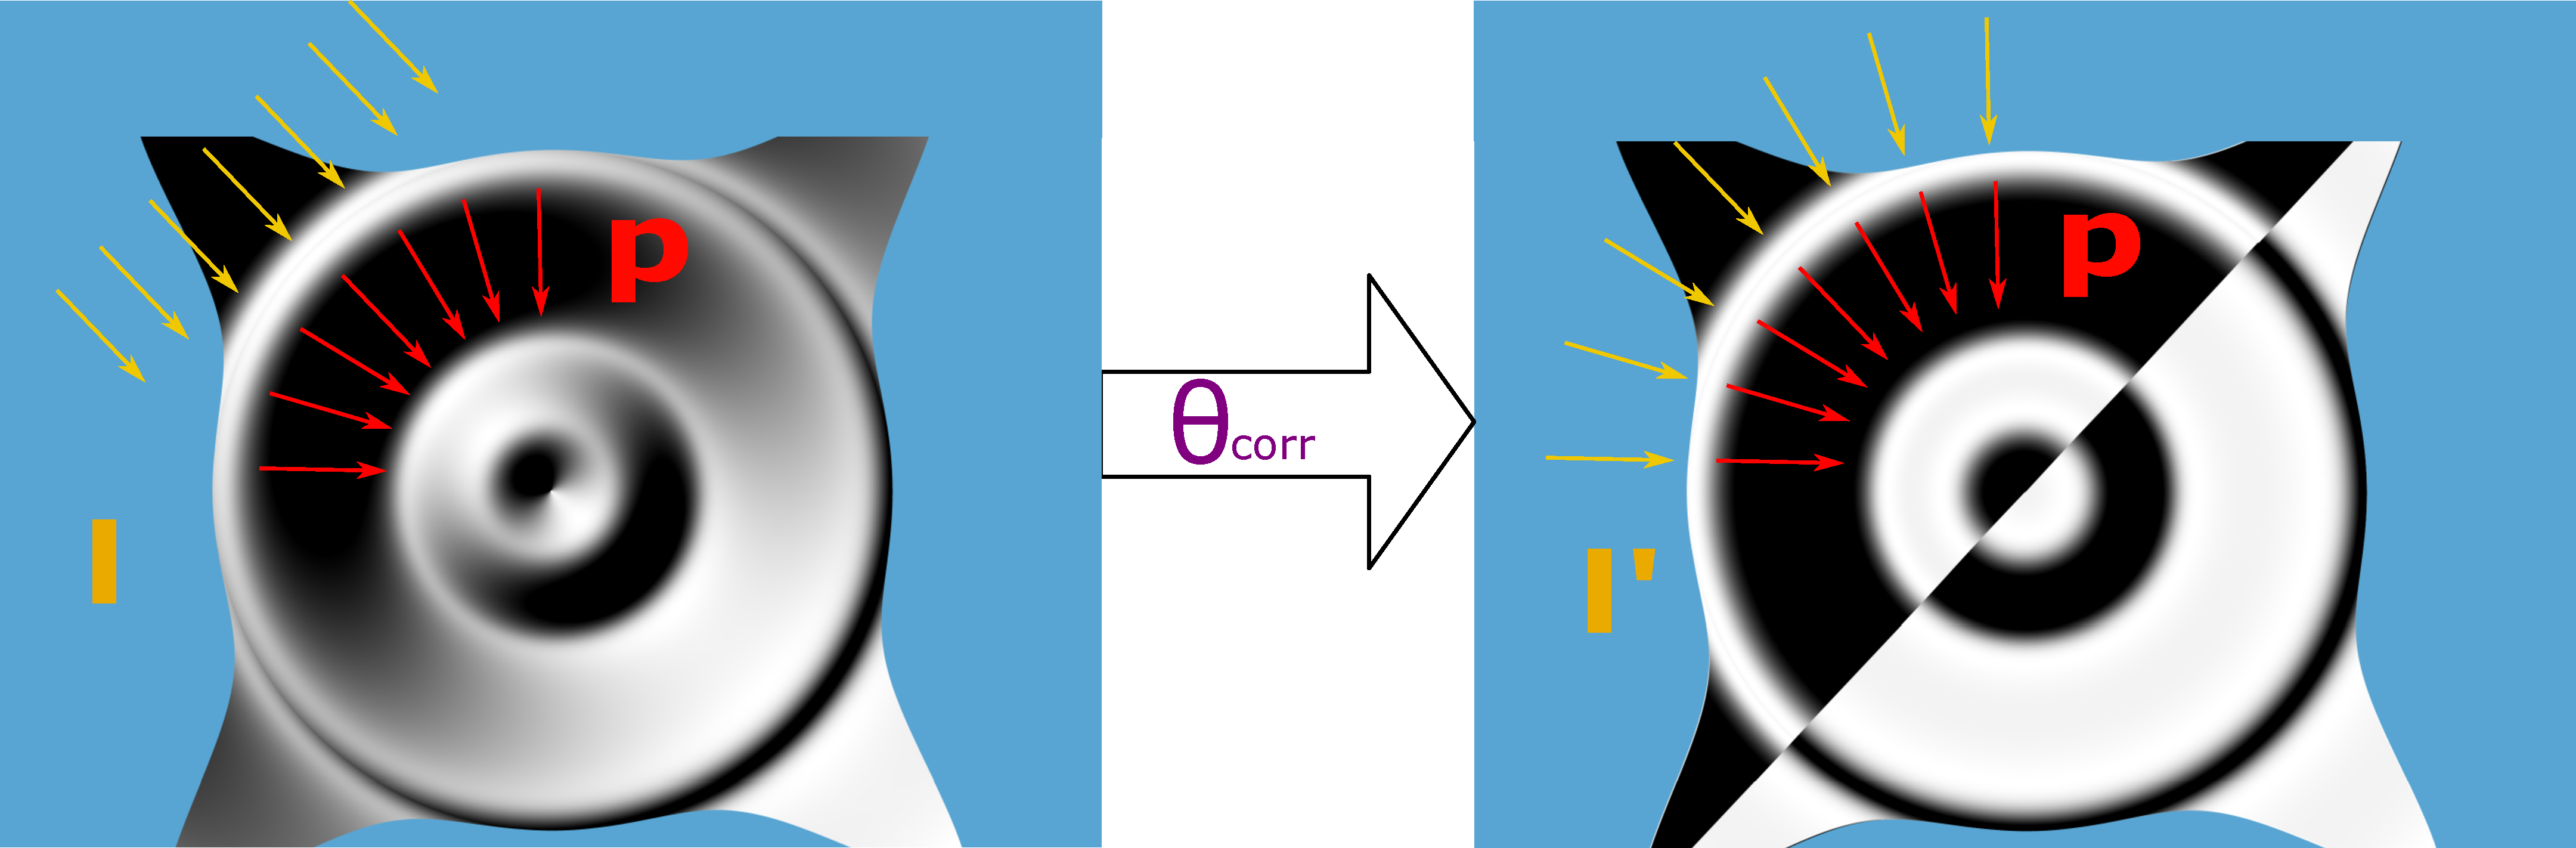
\includegraphics[width=1.0\linewidth]{Schema/correction_light_v3.pdf}
\end{center}


\note{\textbf{Transition} :  Ainsi , voici ce qu'on obtient en ... .\\
\textbf{Mots clés} :Fonctionne mais grosse discontinuité  \\
\begin{center}
\insertslideintonotes{0.7}
\end{center}}	
	



\end{frame}




\begin{frame}{Gestion des discontinuités}

\begin{center}
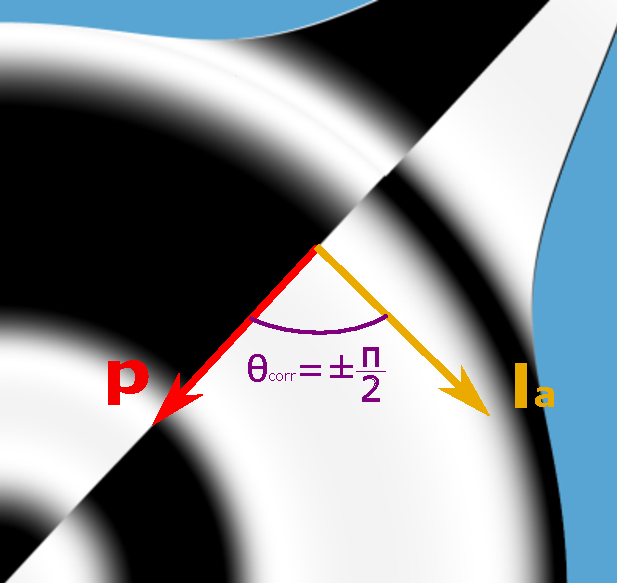
\includegraphics[width=0.6\linewidth]{Schema/orientationTheta_Image_discontinue_1.pdf}
\end{center}

\note{
\textbf{Transition} :  Elle se produit quand ... .\\
\textbf{Mots clés} :Angle droit entre azimut et pente  \\
\begin{center}
\insertslideintonotes{0.7}
\end{center}}	
	


\end{frame}


\begin{frame}{Gestion des discontinuités}

\begin{center}
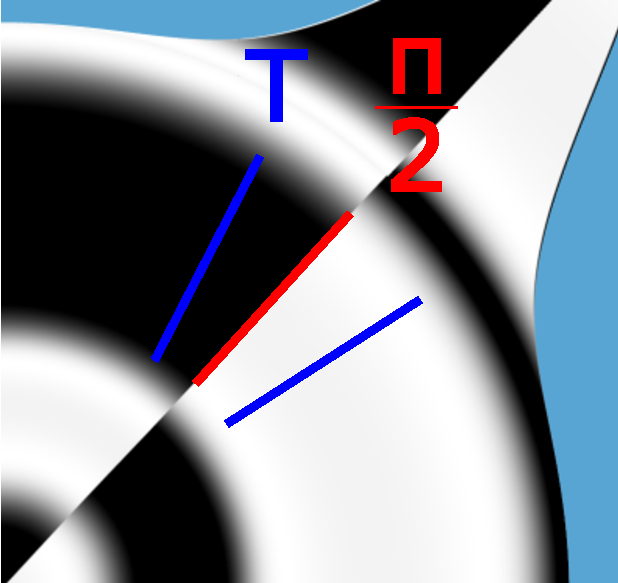
\includegraphics[width=0.6\linewidth]{Schema/orientationTheta_Image_discontinue_2.pdf}
\end{center}

\note{
\textbf{Transition} :  Pour corriger ... .\\
\textbf{Mots clés} :Introduit T , une limite  \\

\begin{center}
\insertslideintonotes{0.7}
\end{center}}	
	

\end{frame}


\begin{frame}{Gestion des discontinuités}

\begin{center}
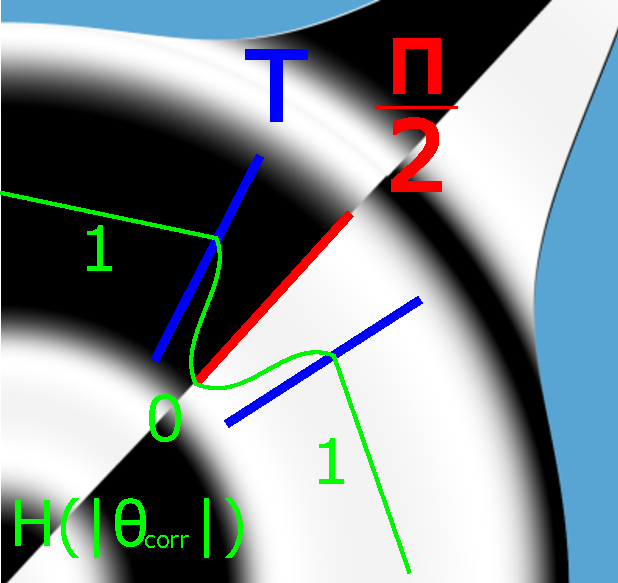
\includegraphics[width=0.6\linewidth]{Schema/orientationTheta_Image_discontinue_3.pdf}
\end{center}
\note{
\textbf{Transition} :  Ensuite ... .\\
\textbf{Mots clés} :Défini H , une spline entre T et $\frac{\pi}{2}$ \\

\begin{center}
\insertslideintonotes{0.7}
\end{center}}	
	


\end{frame}


\begin{frame}{Gestion des discontinuités}

\begin{center}
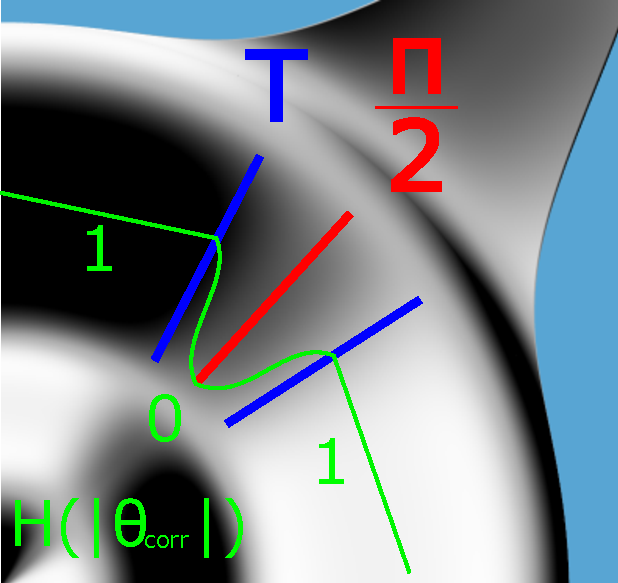
\includegraphics[width=0.6\linewidth]{Schema/orientationTheta_Image_discontinue_4.pdf}
\end{center}

\note{
\textbf{Transition} :  De cette manière on obtient  ... .\\
\textbf{Mots clés} :Transition plus légère \\
\begin{center}
\insertslideintonotes{0.7}
\end{center}}	
	

\end{frame}






\begin{frame}{Gestion des discontinuités} % SAVE : https://www.desmos.com/calculator/aadi3cyiix
\begin{center}
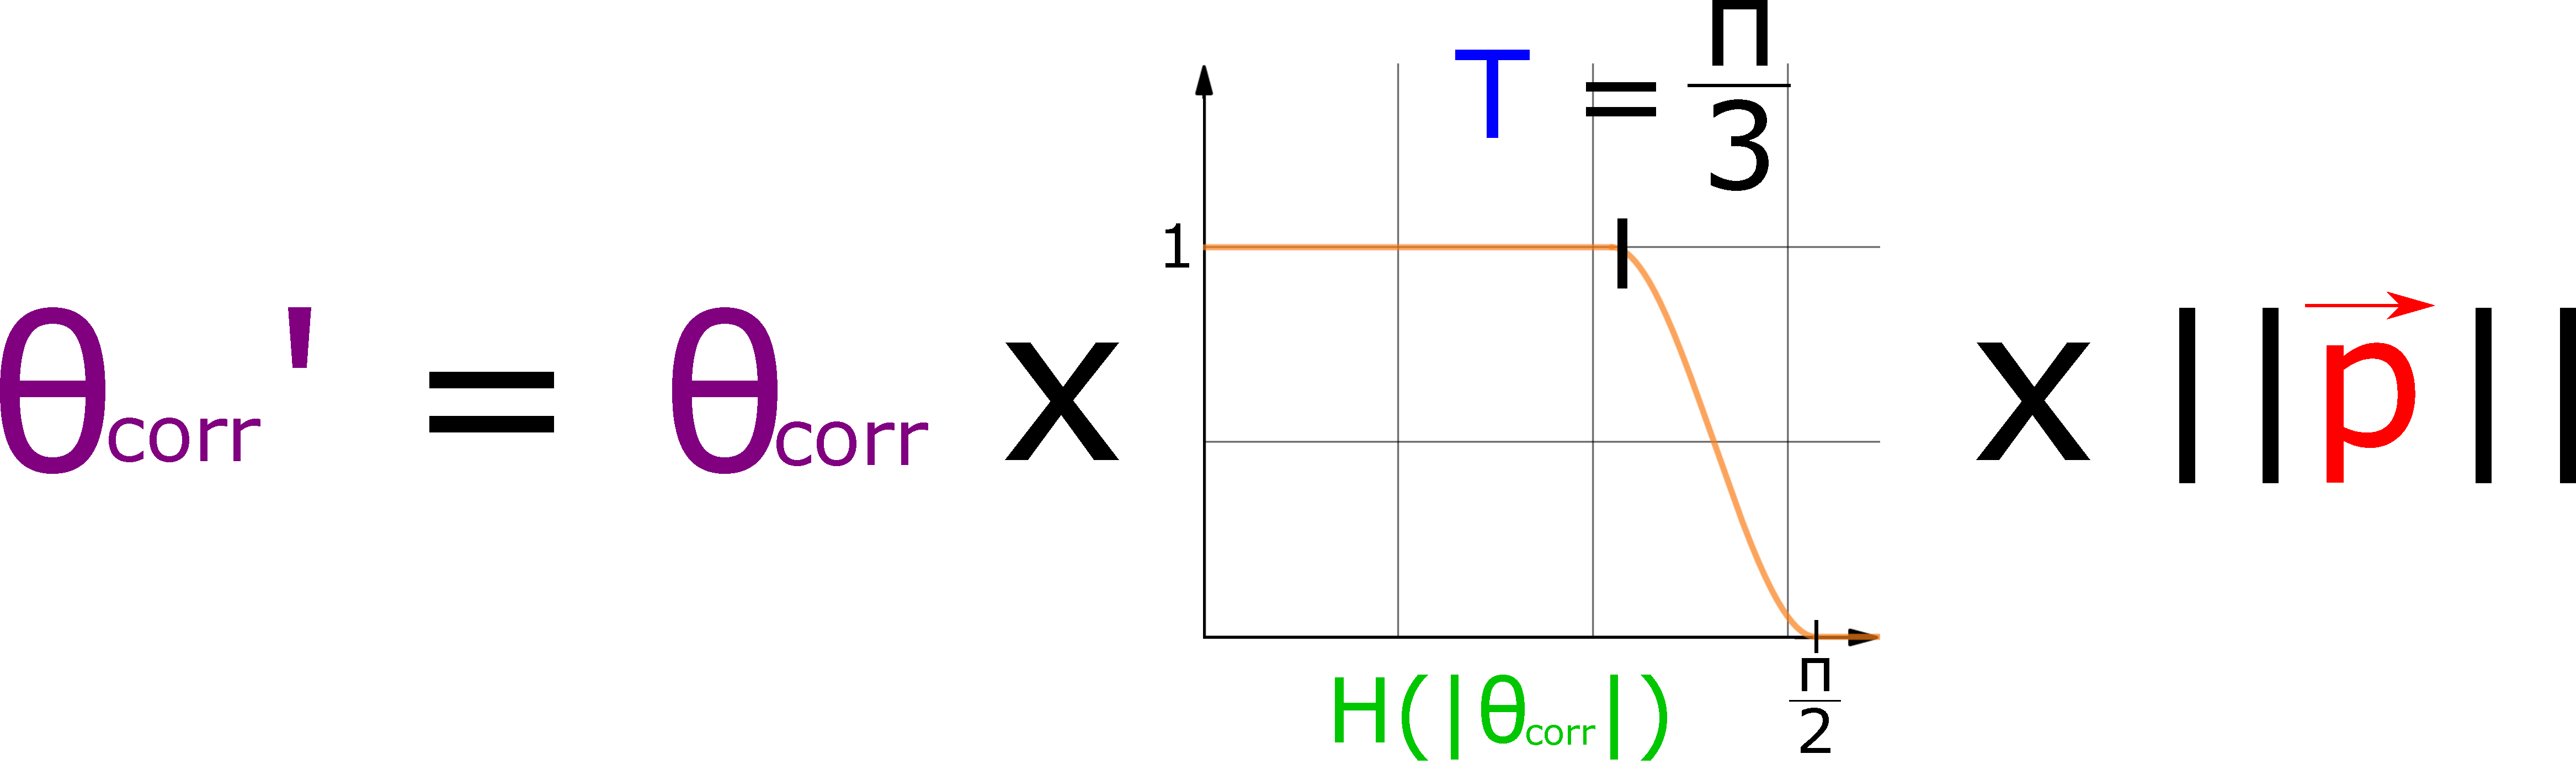
\includegraphics[width=0.9\linewidth]{Schema/smooth-step.pdf}
\end{center}

\note{
\textbf{Transition} : Ainsi le formule est  .\\
\textbf{Mots clés} : T fixe arbitrairement à $\frac{\pi}{3}$ \\
Bon compromis entre \\
Norm P pour aucune correction quand c'est plat \\

\begin{center}
\insertslideintonotes{0.7}
\end{center}}	
\end{frame}


\begin{frame}{Correction finale}

\begin{center} 
        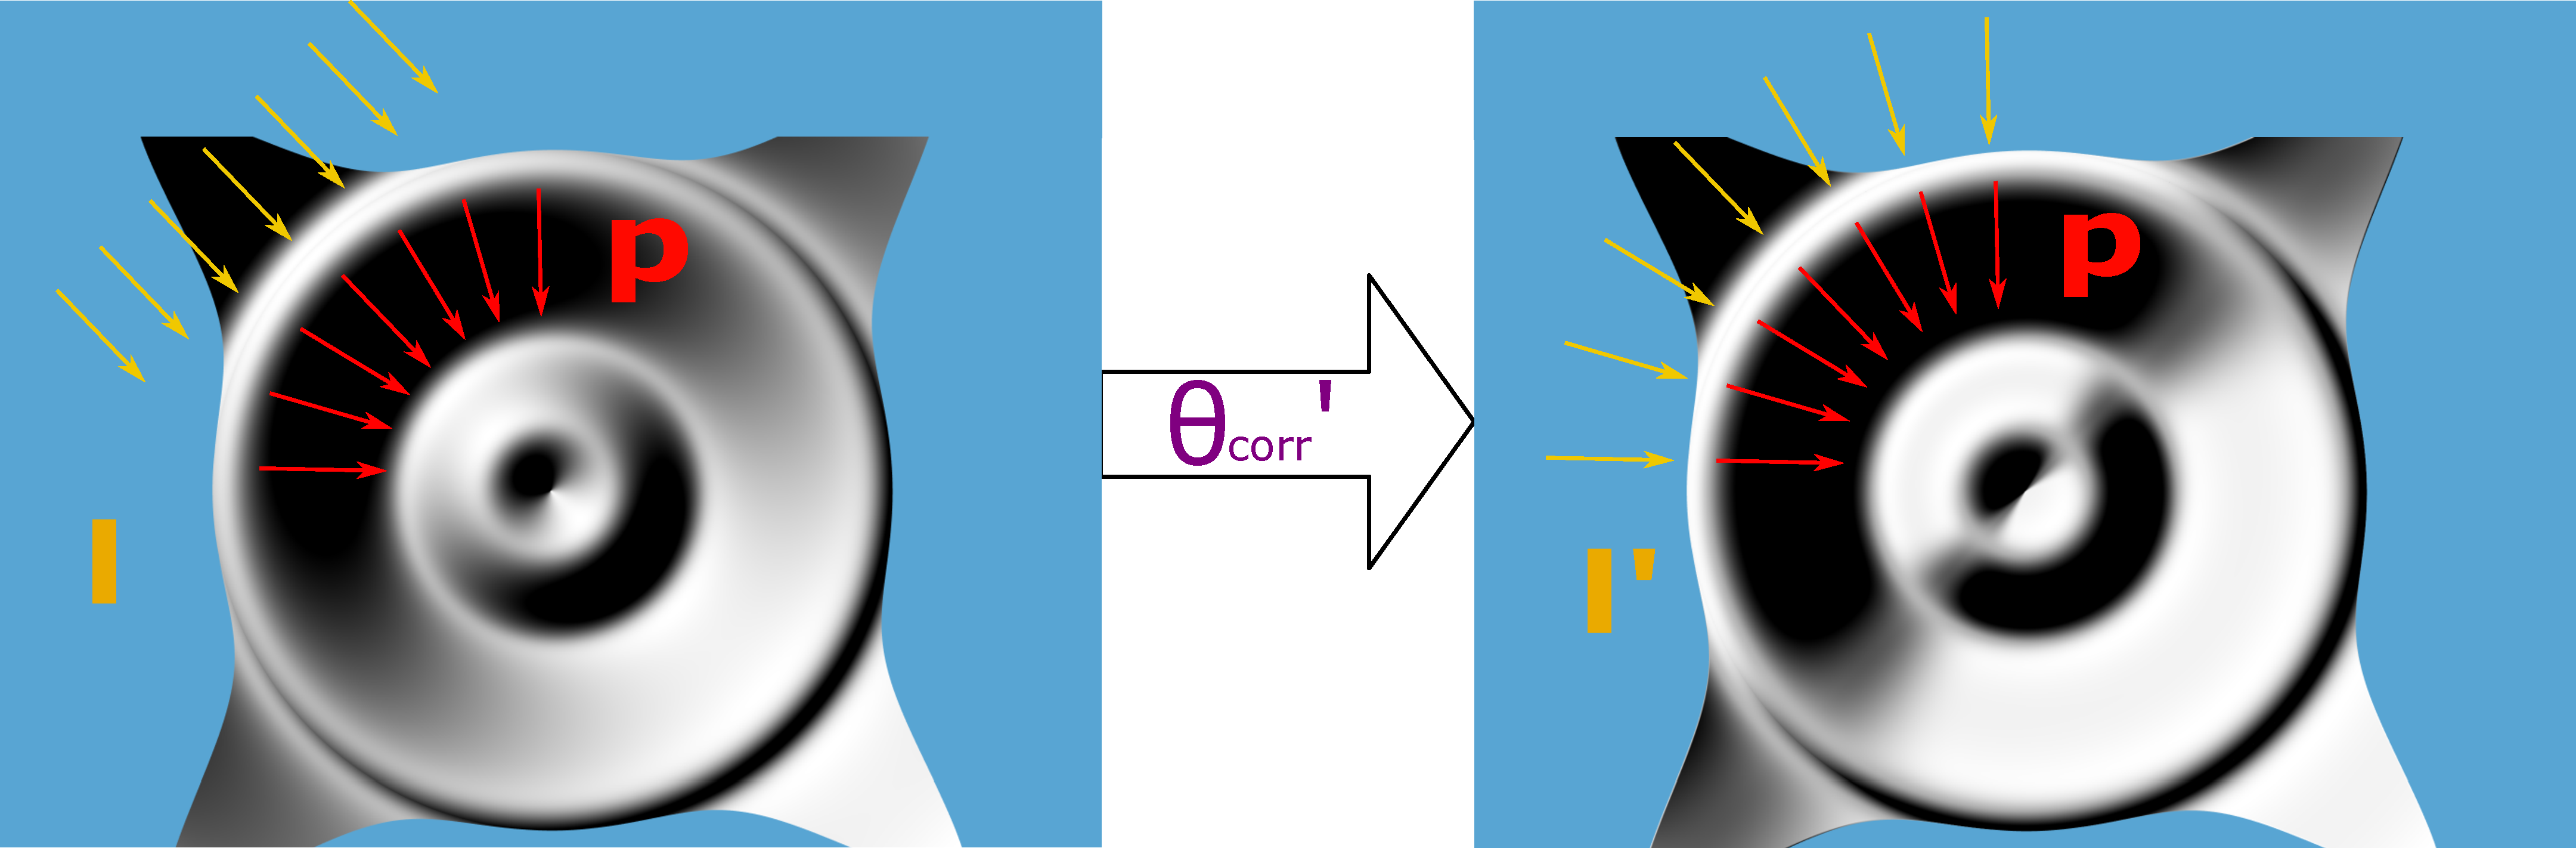
\includegraphics[width=1.0\linewidth]{Schema/correction_light_v2.pdf}
\end{center}


\note{
\textbf{Transition} : Quand on applique $\theta'$  .\\
\textbf{Mots clés} : -\\
\begin{center}
\insertslideintonotes{0.7}
\end{center}}	
	


\end{frame}




\begin{frame}{Résultats sur un terrain}
\begin{center}
    \begin{minipage}[t]{0.4\linewidth}
    \begin{center}
    	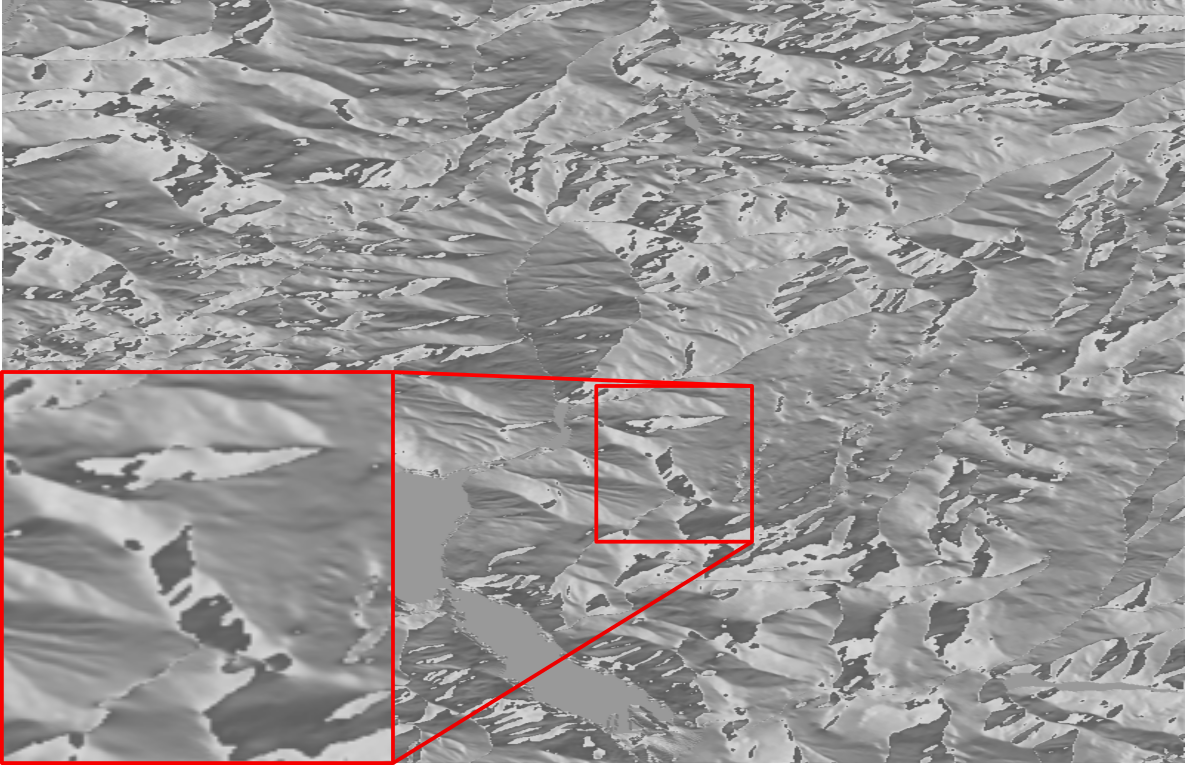
\includegraphics[width=0.9\linewidth]{Resultats/theta_discontinu.png}~\\
 		\textit{$\theta_{corr}$ en niveau de gris}\\  
    	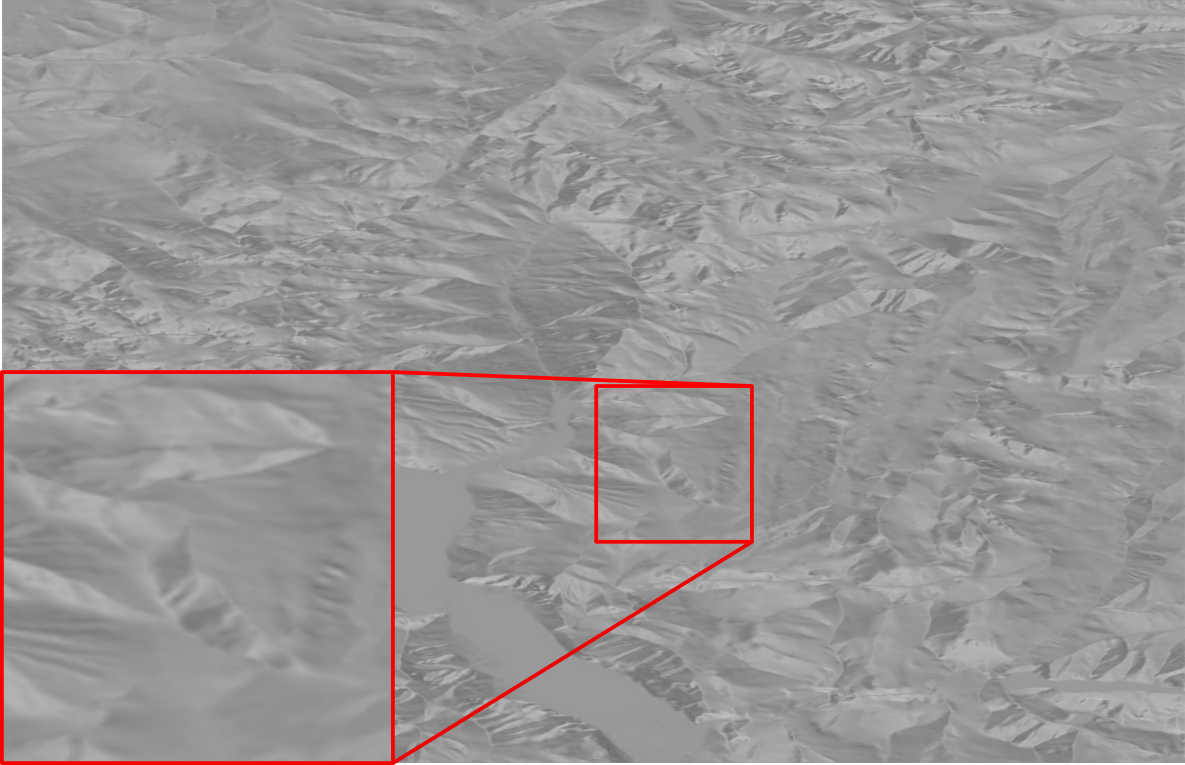
\includegraphics[width=0.9\linewidth]{Resultats/theta_continu.png}~\\
 		\textit{$\theta_{corr}'$ en niveau de gris}
    \end{center}
    \end{minipage}
	\hspace{0.2cm}
    \begin{minipage}[t]{0.4\linewidth}
    \begin{center}
    	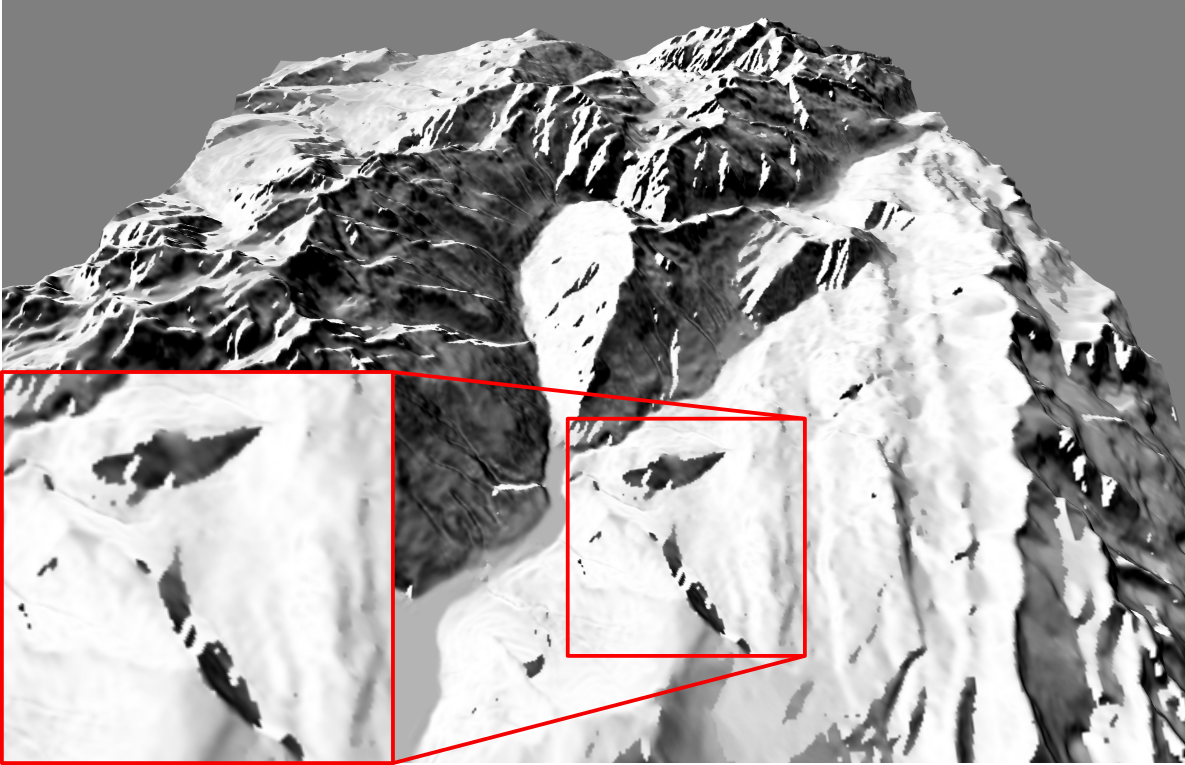
\includegraphics[width=0.9\linewidth]{Resultats/ombrage_discontinue.png}~\\
 		\textit{Illumination avec $\theta_{corr}$}
        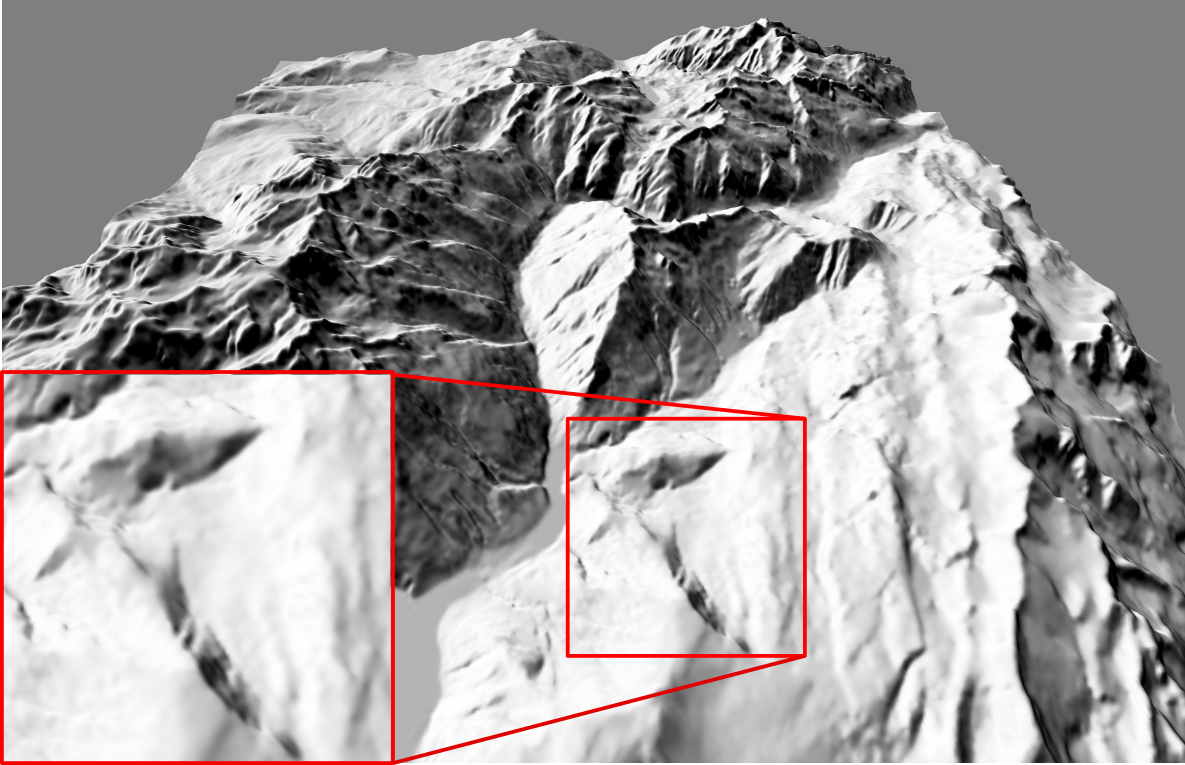
\includegraphics[width=0.9\linewidth]{Resultats/ombrage_continue.png}~\\
 		\textit{Illumination avec $\theta_{corr}'$}
    \end{center}
    \end{minipage}
\end{center}

\note{
\textbf{Transition} : Et sur un terrain   .\\
\textbf{Mots clés} : Haut Discontinu - Bas continu\\
\textbf{Temps :} 13'30 min MAX .\\
\begin{center}
\insertslideintonotes{0.7}
\end{center} }

\end{frame}
% Jon : avant après meilleur que uniquement après ? zoom aprés animations




%[Schema correction local ]
%[Formule calcule de l'angle ]
%[Resultat discontinu]
%[theta * courbe smooth * courbe normS  avec la formule de correction en dessous]
%[Resultat continue]
\subsection*{Multi-echelle}
\begin{frame}{Multi-échelle }
\begin{onlyenv}<1>
\begin{center}
    \begin{minipage}[c]{0.45\linewidth}
    \begin{center}
    	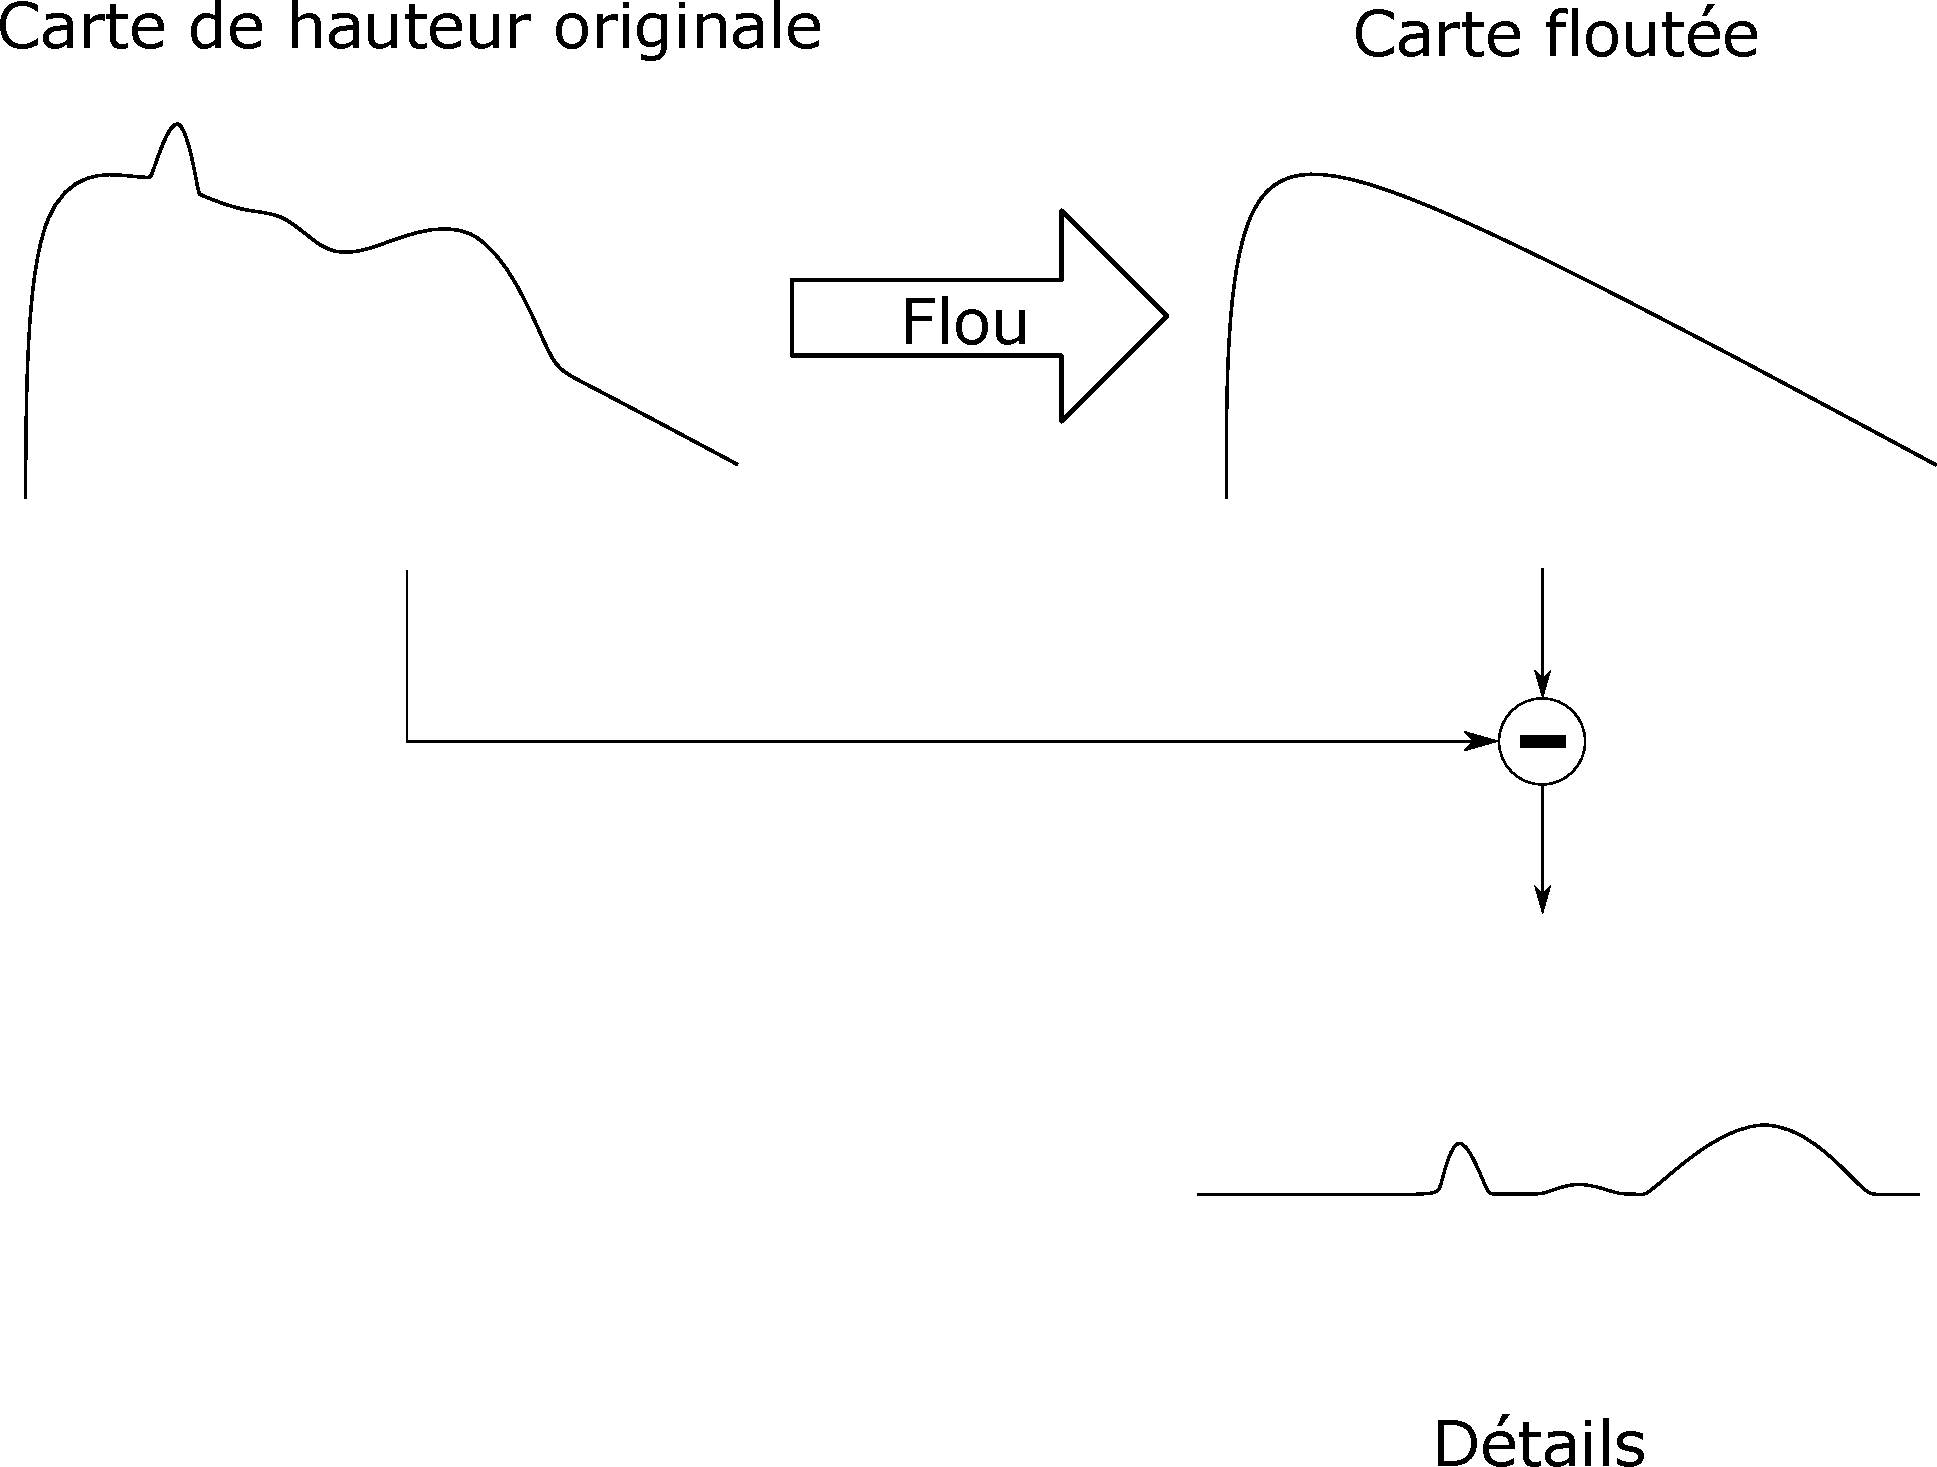
\includegraphics[width=1.0\linewidth]{Schema/pyramide_Laplace_schema.pdf}\\
 		\textit{Pyramide Laplacienne 1D}
    \end{center}
    \end{minipage}
    \hspace{0.2cm}
    \begin{minipage}[c]{0.45\linewidth}
    \begin{center}
    	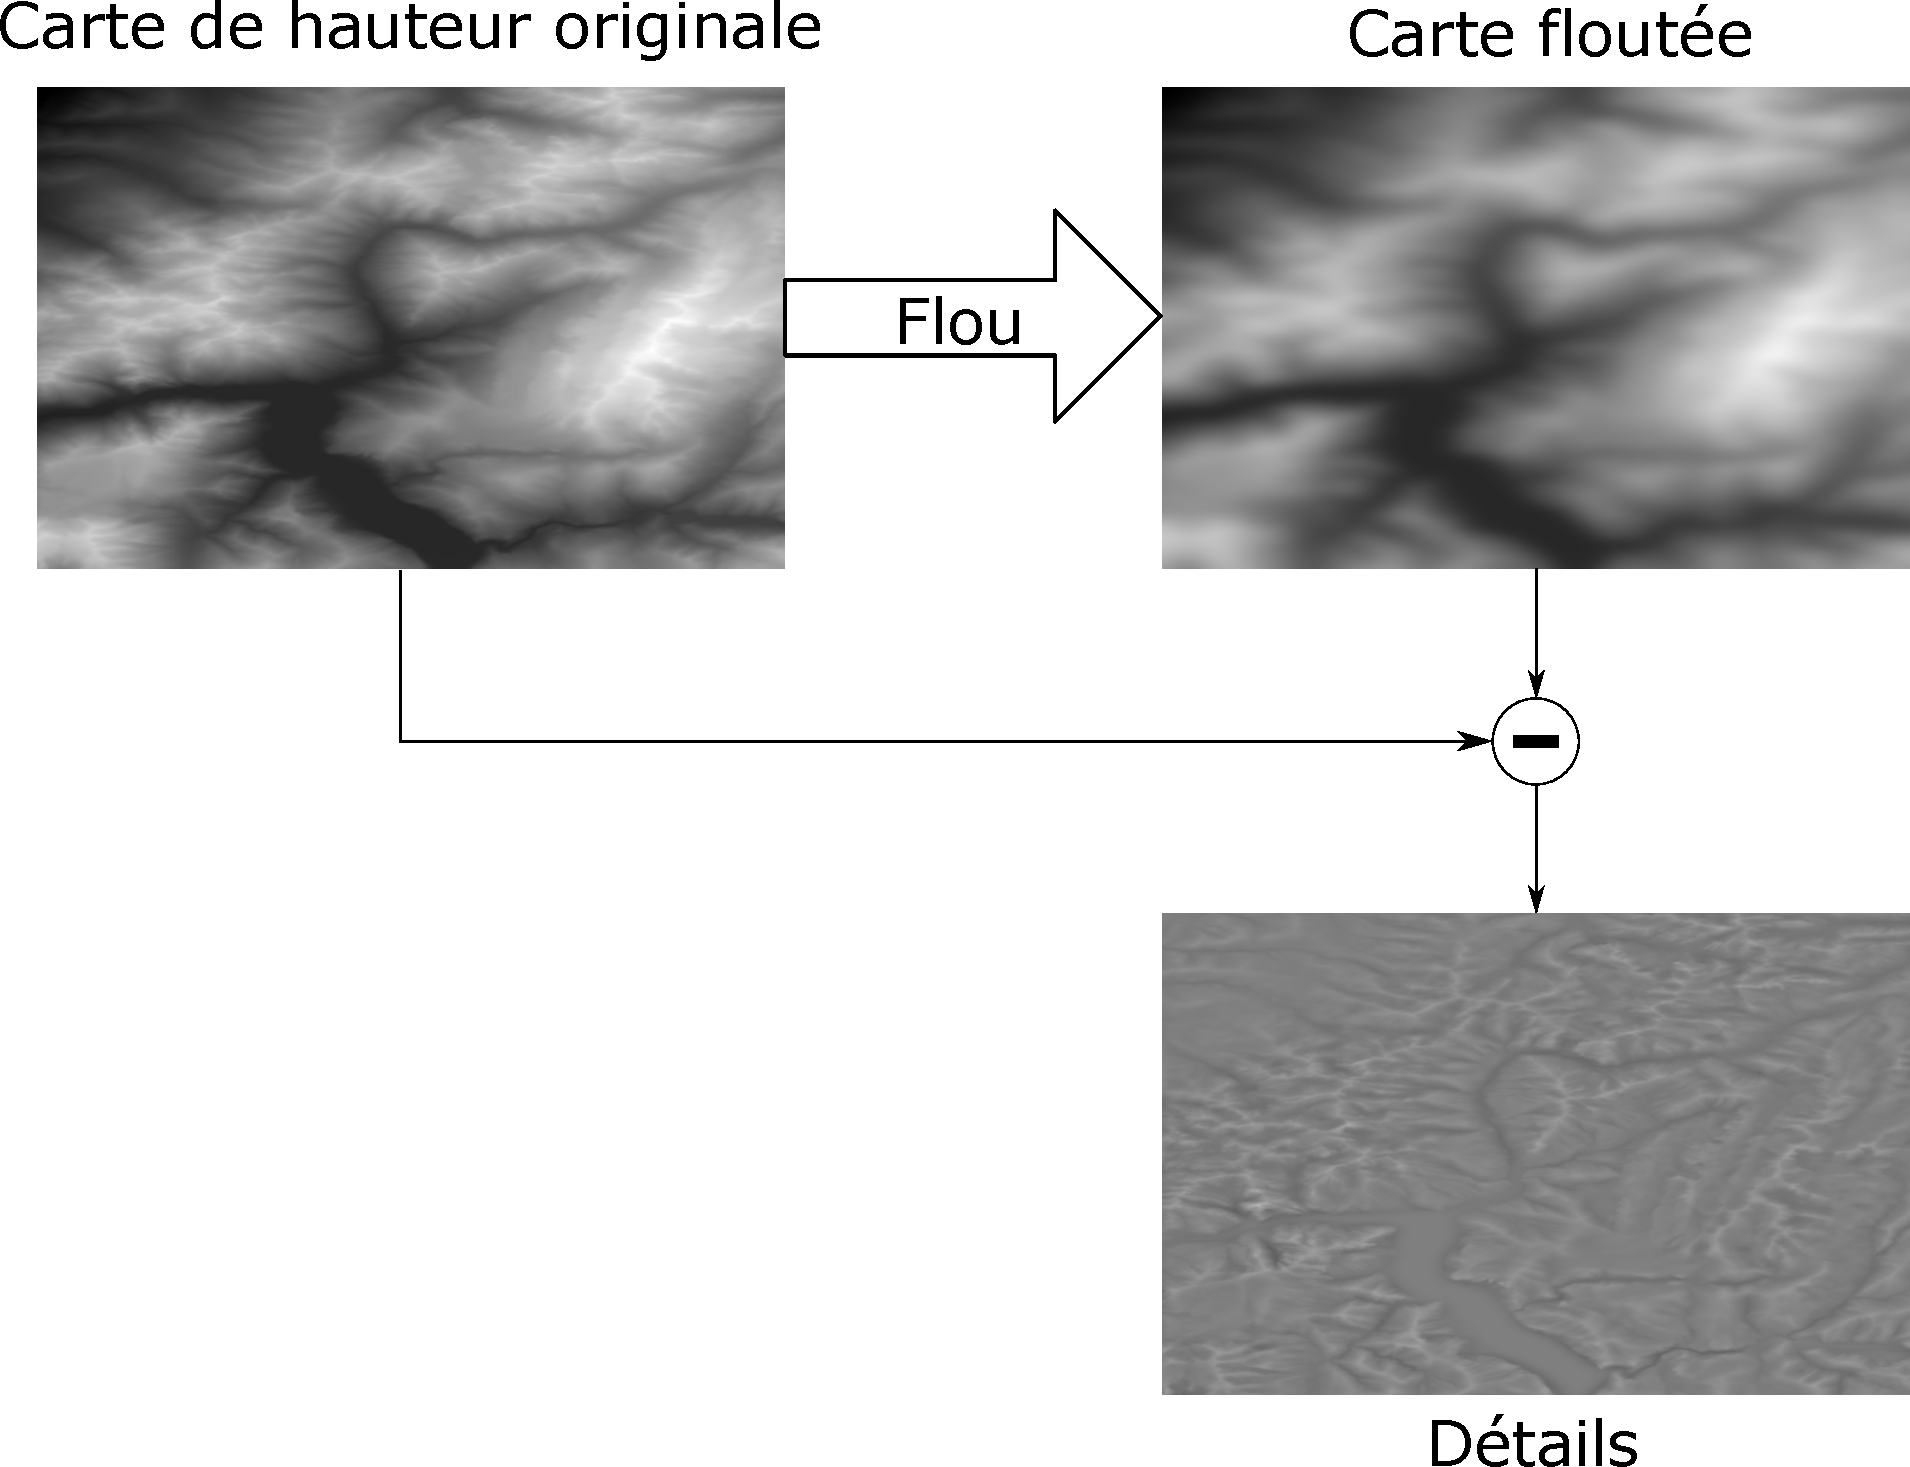
\includegraphics[width=1.0\linewidth]{Schema/pyramide_Laplace_image.pdf}\\
 		\textit{Pyramide Laplacienne 2D}
    \end{center}
    \end{minipage}

\end{center}
\end{onlyenv}
\begin{onlyenv}<2>
\begin{center}
    
    	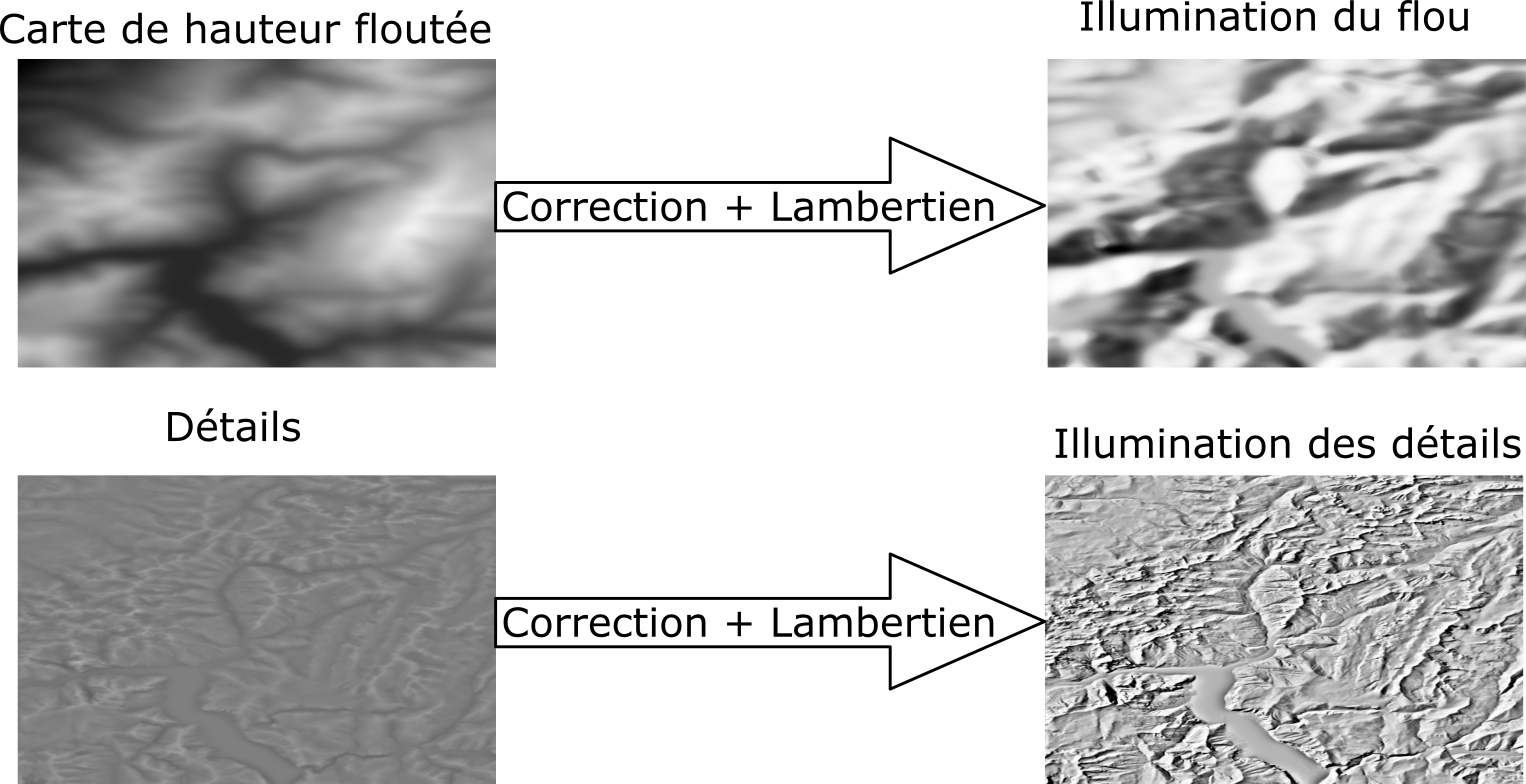
\includegraphics[width=1.0\linewidth]{Schema/pyramide_Laplace_image_extended_short.png}\\
 	
\end{center}
\end{onlyenv}

\note{
\textbf{Transition} : Maintenant qu'on vu la correction local , passe sur plusieurs échelle. \\
\textbf{Mots clés} : Correction une echelle marche pas \\
Séparation des aspérités \\
Correction et illumination indépendante \\

\begin{center}
\insertslideintonotes{0.7}
\end{center}}	
	


\end{frame}


\subsection*{Fusion}
\begin{frame}{Fusion}
\begin{center}
	\begin{minipage}[t]{0.32\linewidth}
    \begin{center}
    	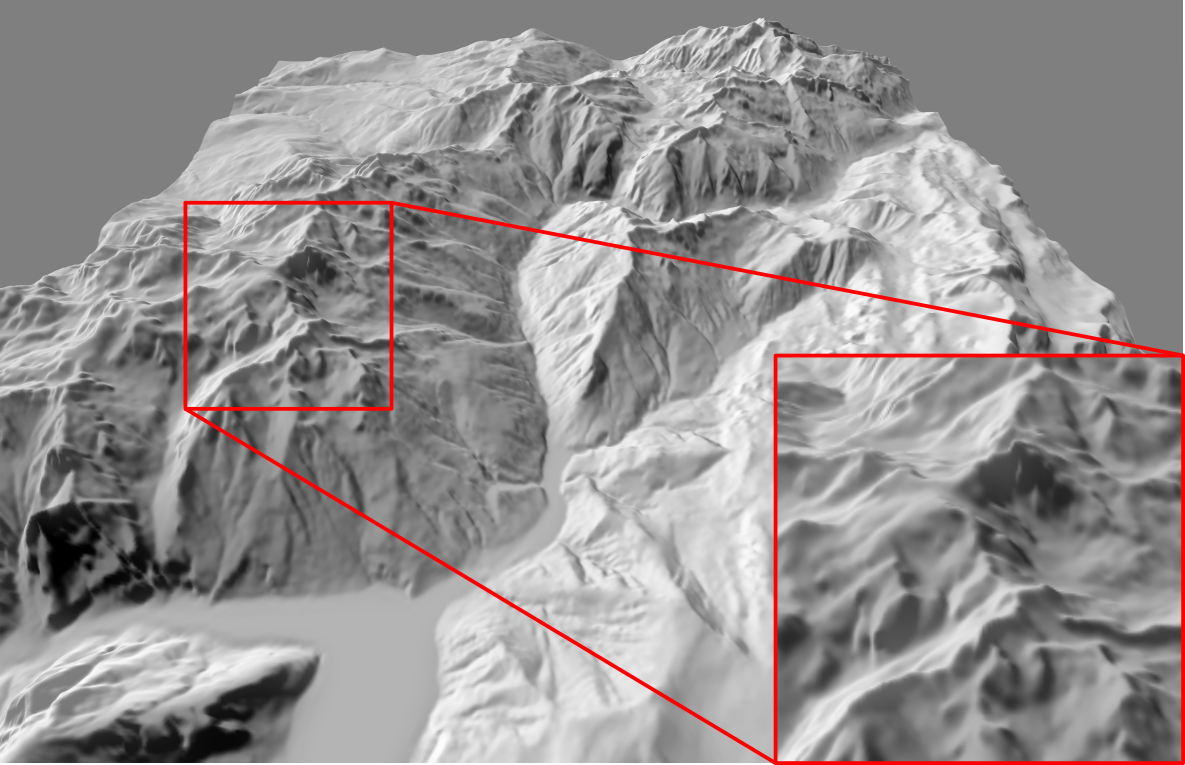
\includegraphics[width=1.0\linewidth]{Resultats/ShadeLineaire.png}\\
 		\textit{Interpolation linéaire}
    \end{center}
    \end{minipage}
    \begin{minipage}[t]{0.32\linewidth}
    \begin{center}
    	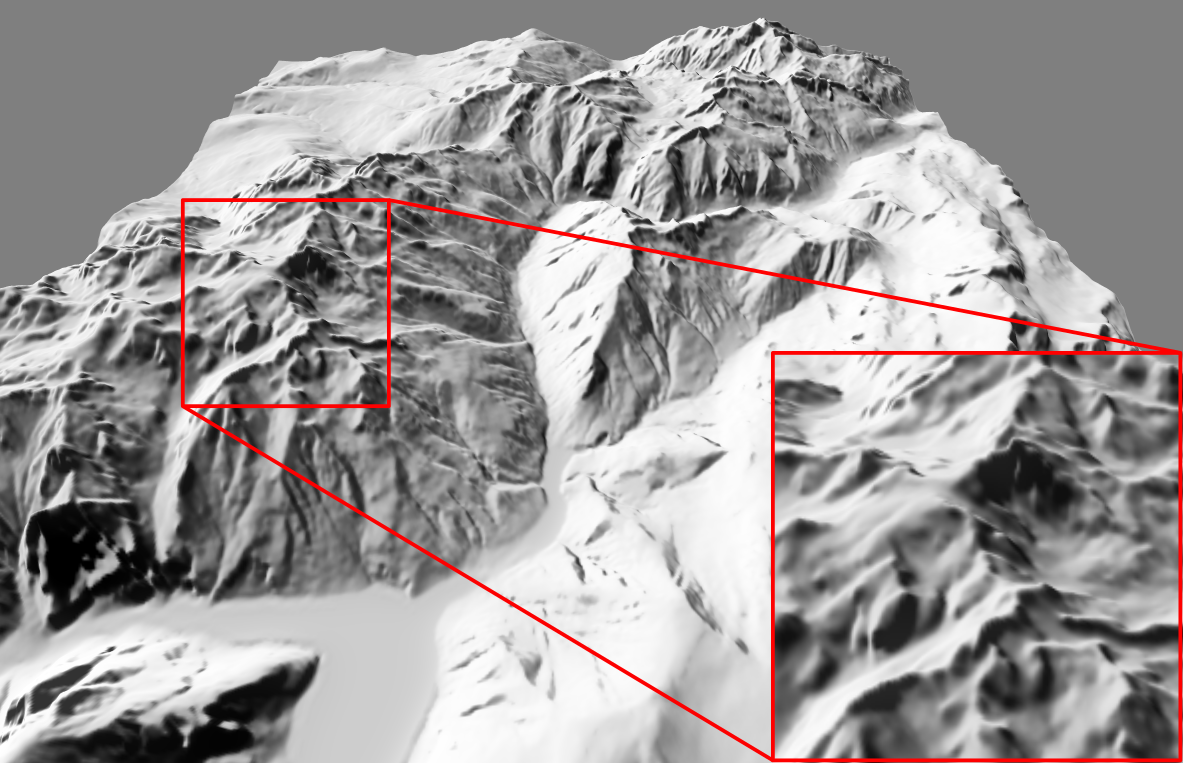
\includegraphics[width=1.0\linewidth]{Resultats/ShadeOverlay.png}\\
 		\textit{Overlay de Gimp et photoshop}
    \end{center}
    \end{minipage}
        \begin{minipage}[t]{0.32\linewidth}
    \begin{center}
    	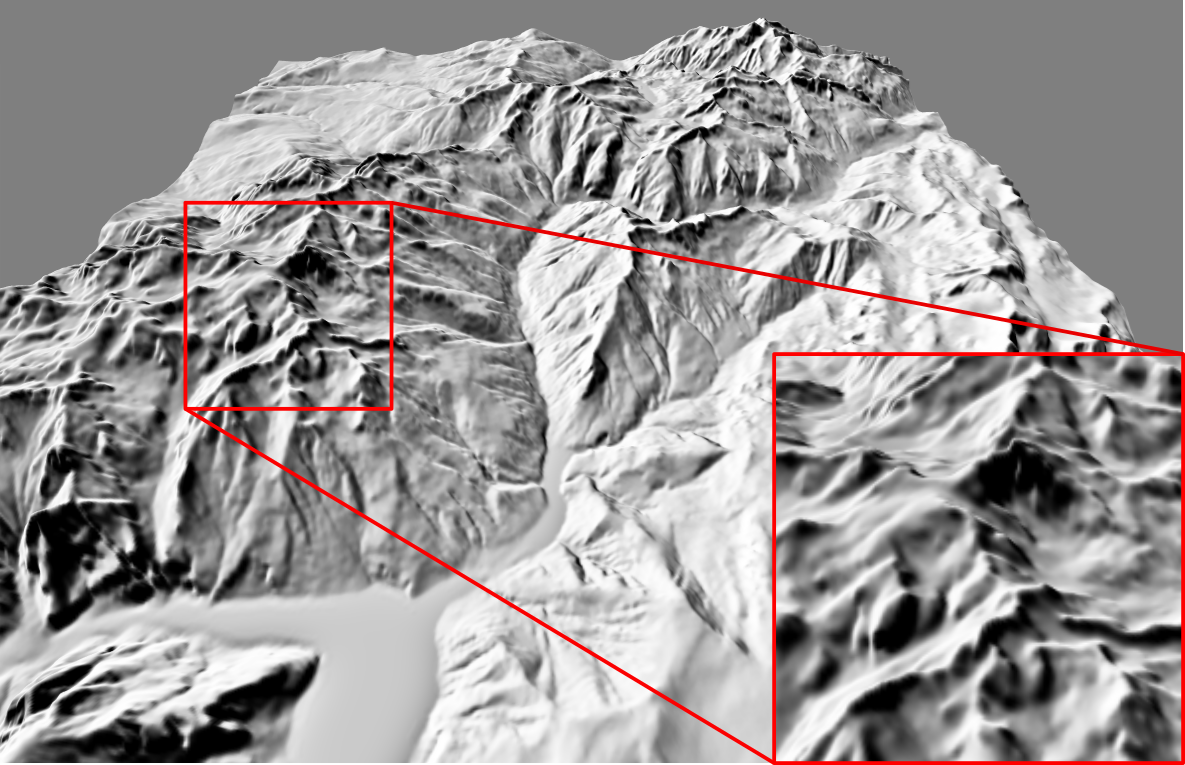
\includegraphics[width=1.0\linewidth]{Resultats/ShadeWatercolor.png}\\
 		\textit{Mélange aquarelle de [Bousseau et al. 2006]}\\
 		\textbf{Méthode choisie}
    \end{center}
    \end{minipage}
    \end{center}
    
\note{
\textbf{Transition} : Il faut ensuite fusionner ces illuminations
\\
\textbf{Mots clés} :Interpolation linaire non adapter --> pas assez de contraste  \\
Overlay -> plus contrasté  --> perte quand la partie flou est blanche\\
aquarelle -> corrige ce probleme. \\
\begin{center}
\insertslideintonotes{0.7}
\end{center}}	
	

\end{frame}



\subsection*{Ajout des ombres portées}
\begin{frame}{Ombre portées}
	Fusion des ombres : 
    \begin{equation}
		P_{final} = P_{illumination} . \frac{P_{ombresportees}+1}{2}
	\end{equation} 
    \begin{center}
    	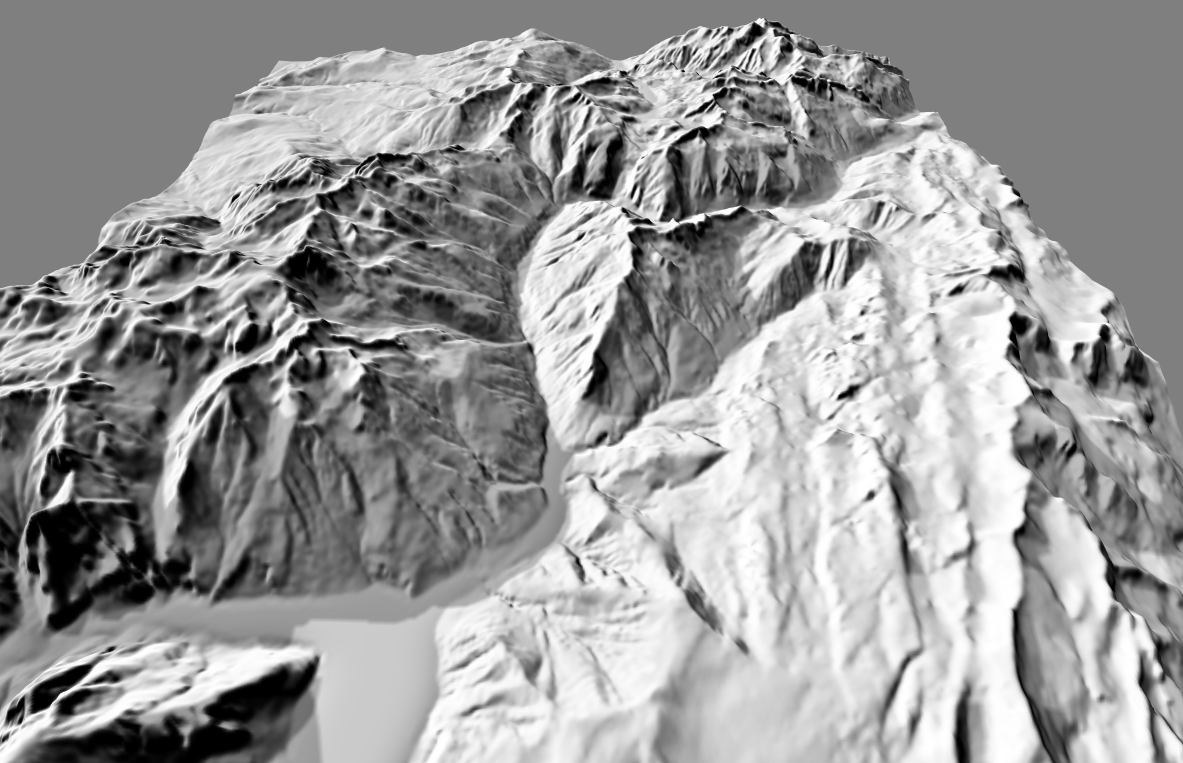
\includegraphics[width=0.5\linewidth]{Resultats/shadow_shade.png}\\
 		\textit{Illumination + Ombre portées }
    \end{center}
    
    
    \note{
	\textbf{Transition} : Et pour terminer , on ajoute des ombres portées\\    
    \textbf{Mots clés} : RayMarching , morpho mathématique \\
    Valeur entre 0.5 et 1, pour ne pas effacer l'illumination  \\
\textbf{Temps :} 15'30 min MAX . 	\\
\begin{center}
\insertslideintonotes{0.7}
\end{center}}
\end{frame}




\startsection{Résultats}
\subsection*{Notre méthode d'illumination}
\begin{frame}{Résultats}
\begin{center}
	\begin{minipage}[t]{0.32\linewidth}
    \begin{center}
    	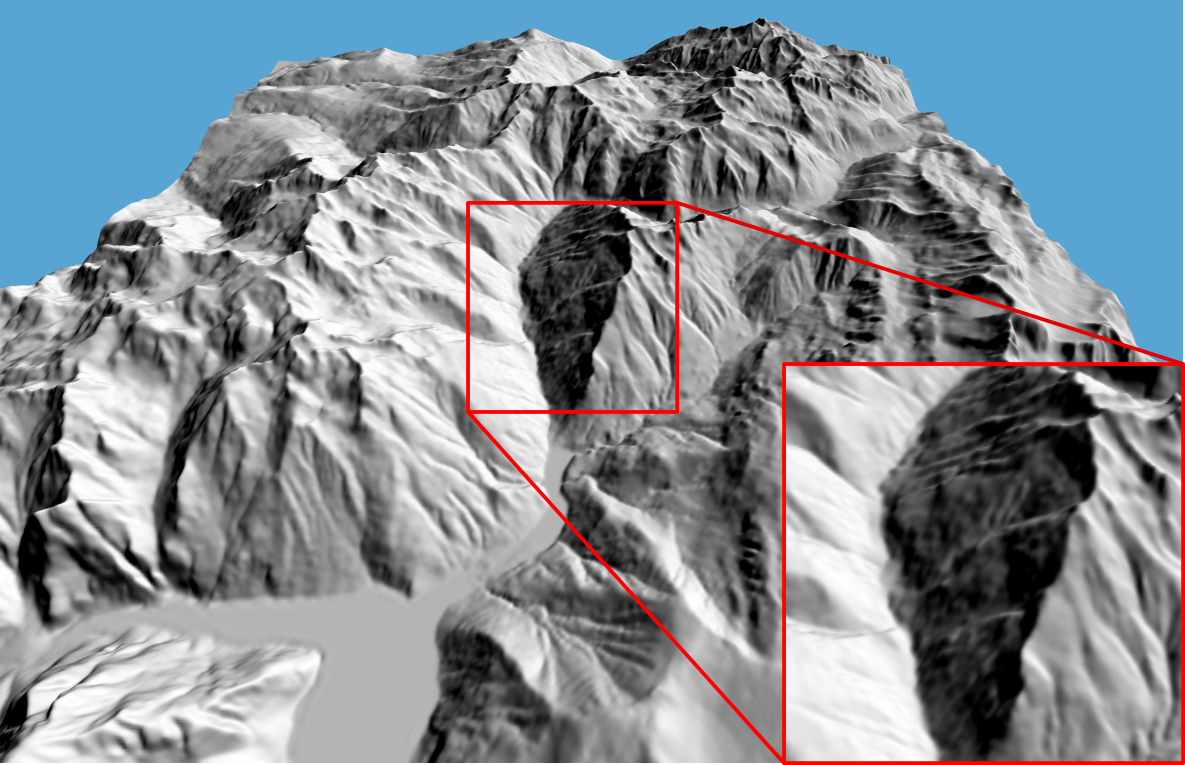
\includegraphics[width=1.0\linewidth]{Resultats/lambertien.png}\\
 		\textit{Lambertien classique}
    \end{center}
    \end{minipage}
    \begin{minipage}[t]{0.32\linewidth}
    \begin{center}
    	\includegraphics[width=1.0\linewidth]{Resultats/ombrage.png}\\
 		\textit{Notre méthode}
    \end{center}
    \end{minipage}
        \begin{minipage}[t]{0.32\linewidth}
    \begin{center}
    	\includegraphics[width=1.0\linewidth]{Resultats/ombre_portee.png}\\
 		\textit{Notre méthode avec les ombres portées}
    \end{center}
    \end{minipage}
    \end{center}
    
    
\visible<2->{    
\textbf{Entretien avec Arthur Novat}
\begin{itemize}
\item Plus de zone bouchée.
\item Suffisamment de variation dans les zones éclairées.
\item Ce qu'il imagine avec une carte d'état major.
\end{itemize}
}


    \note{
\textbf{Transition} : Si on compare avec un Lambertien  \\    
    \textbf{Mots clés} : On perçois plus de variation \\
    Quand on demande à Arthur son avis \\

\begin{center}
\insertslideintonotes{0.7}
\end{center} }	

\end{frame}




\begin{frame}{Colorisation}
\subsection*{Colorisation avec les couleurs de Novat}
\begin{center}
	\begin{minipage}[t]{0.32\linewidth}
    \begin{center}
    	\includegraphics[width=1.0\linewidth]{Resultats/aquarelle.png}\\
 		\textit{Mélange aquarelle de [Bousseau et al. 2006]}
    \end{center}
    \end{minipage}
    \begin{minipage}[t]{0.32\linewidth}
    \begin{center}
    	\includegraphics[width=1.0\linewidth]{Resultats/colorMap.png}\\
 		\textit{Rampe de couleur dégradé}
    \end{center}
    \end{minipage}
        \begin{minipage}[t]{0.32\linewidth}
    \begin{center}
    	\includegraphics[width=1.0\linewidth]{Resultats/cel_shading.png}\\
 		\textit{Cel-shading}
    \end{center}
    \end{minipage}
    \end{center}
    
    
    \note{
\textbf{Transition} : Enfin , on ajoute de la couleur pour être plus proche\\    
    \textbf{Mots clés} : On utilise les couleurs fourni Arthur Novat \\
    \textbf{Temps :} 17'30 min MAX .\\
	
\begin{center}
\insertslideintonotes{0.7}
\end{center}}	
    
    
\end{frame}






\startsection{Limitations et travaux futurs}
\subsection*{Limitations}
\begin{frame}{Limitations}




\visible<1->{
\begin{itemize}
\item<1-> Avoir un nombre N d'échelles.
\begin{itemize}
\item<2-> Couche d'illumination intermédiaire. 
\item<2-> Comment les fusionner ?
\end{itemize}
\item<3-> Améliorer les ombres portées.
\item<4-> Faire une colorisation plus proche du style Novat.
\end{itemize}
}
    \note{
	\textbf{Transition} : Pour finir , on va voir les limitations de notre méthode et les travaux futures \\     
    \textbf{Mots clés} : 
    \begin{itemize}
    \item Multi-echelle : -
    \item Ombres portées : + exploiter morpho, Elevation local
    \item Couleur : + artistique , prendre en compte l'altitude.  
    \end{itemize}
	
\begin{center}
\insertslideintonotes{0.7}
\end{center} }	
    
\end{frame}
\subsection*{Travaux futurs}
\begin{frame}{Travaux futurs}
\visible<1->{
\begin{itemize}
\item<1-> Fusionner avec la déformation de la montagne.
\item<2-> Faire le reste des éléments.
\end{itemize}
}
\begin{center}
\only<1>{\includegraphics[width=0.6\textwidth]{Images/AlpeHuez.png}}
\only<2>{\includegraphics[width=0.6\textwidth]{Images/PN_Elements_2.png}}
\end{center}
    
    \note{
	\textbf{Transition} : Enfin les travaux futurs \\    
    \textbf{Mots clés} : -\\
\begin{center}
\insertslideintonotes{0.7}
\end{center} }	
    

\end{frame}

\begin{frame}{Conclusion}
Deux contributions : 
\begin{itemize}
\item Étude du style de Pierre Novat.
\item Calcul d'une illumination expressive $\rightarrow$ plus générique. 
\end{itemize}
~\\
\textbf{Principale difficulté :} 
\begin{itemize}
\item Transmission du savoir.
\item Langage différent. 
\end{itemize}


    \note{
\textbf{Transition} : Pour conclure\\    
    \textbf{Mots clés} :adaptable à d'autre panorama , Novat est une porte d'entrée pour ce type de rendu \\
	\textbf{Transition} : MERCI  \\
	\textbf{Temps : } Fin 20'30 min MAX\\
\begin{center}
\insertslideintonotes{0.7}
\end{center} }	
    


\end{frame}

\begin{frame}{Merci}
\begin{center}
\textbf{Des questions ?} 
\end{center}

\begin{textblock*}{30mm}[0,0](80mm,50mm)

\includegraphics[width=25mm]{Images/simon.jpg}

\end{textblock*}
\end{frame}


\begin{frame}[noframenumbering]{Qu'est-ce que c'est que de dessiner un panorama du point de vue d'Arthur Novat ?}
Représentation imaginaire :
\begin{itemize}
\item Faire aimer la montagne
\item Répond à une demande. 
\end{itemize}
\begin{center}
\begin{minipage}[c]{0.45\linewidth}
Contraintes :
\begin{itemize}
\item Géographiques 
\item Respecter les commanditaires
\item Respecter les habitants
\end{itemize}	
\end{minipage}
\begin{minipage}[c]{0.45\linewidth}
\begin{center}
\includegraphics[width=1.0\textwidth]{Images/AlpeHuez_pistes.png}
\end{center}
\end{minipage}
\end{center}

\end{frame}

\begin{frame}[noframenumbering]{Étape de création d'un panorama}
\begin{enumerate}
\item Prise d'information.
\item Déformation de la montagne.
\item Crayonné. 
\item Ajout des couleurs. 
\end{enumerate}

\begin{center}
    \begin{minipage}[c]{0.45\linewidth}
    \begin{center}
    	\includegraphics[width=1.0\linewidth]{Images/crayonn_.png}
    \end{center}
    \end{minipage}
    \hspace{0.2cm}
    \begin{minipage}[c]{0.45\linewidth}
    \begin{center}
    	\includegraphics[width=1.0\linewidth]{Images/courchevel.png}
    \end{center}
    \end{minipage}

\end{center}
\end{frame}

\begin{frame}[noframenumbering]{Validation}
\begin{onlyenv}<1>
\textbf{Entretien avec Arthur Novat}
\begin{itemize}
\item Plus de zone bouchée.
\item Suffisamment de variation dans les zones éclairées.
\item Ce qu'il imagine avec une carte d'état major
\end{itemize}
\begin{center}
	\begin{minipage}[t]{0.32\linewidth}
    \begin{center}
    	\includegraphics[width=1.0\linewidth]{Resultats/lambertien.png}\\
 		\textit{Lambertien classique}
    \end{center}
    \end{minipage}
    \begin{minipage}[t]{0.32\linewidth}
    \begin{center}
    	\includegraphics[width=1.0\linewidth]{Resultats/ombrage.png}\\
 		\textit{Notre méthode}
    \end{center}
    \end{minipage}
        \begin{minipage}[t]{0.32\linewidth}
    \begin{center}
    	\includegraphics[width=1.0\linewidth]{Resultats/ombre_portee.png}\\
 		\textit{Notre méthode avec les ombres portées}
    \end{center}
    \end{minipage}
    \end{center}
\end{onlyenv}
\begin{onlyenv}<2>
\textbf{Piste d’évaluation quantitative} 
\begin{itemize}
\item Déterminer une corrélation locale.
\item Pas d'information sur la perception globale.
\end{itemize}
\begin{center}
	\begin{minipage}[t]{0.32\linewidth}
    \begin{center}
    	\includegraphics[width=1.0\linewidth]{Resultats/gradient_hauteur.png}\\
 		\textit{Gradient carte de hauteur}
    \end{center}
    \end{minipage}
    \begin{minipage}[t]{0.32\linewidth}
    \begin{center}
    	\includegraphics[width=1.0\linewidth]{Resultats/gradient_lambertien.png}\\
 		\textit{Gradient Lambertien}
    \end{center}
    \end{minipage}
        \begin{minipage}[t]{0.32\linewidth}
    \begin{center}
    	\includegraphics[width=1.0\linewidth]{Resultats/gradient_our.png}\\
 		\textit{Gradient notre méthode}
    \end{center}
    \end{minipage}
    \end{center}
\end{onlyenv}
\begin{onlyenv}<3>
\textbf{Validation finale :} 
\begin{itemize}
\item Reprendre l'étude de [Balzarini et al. 2016].
\item Comparer les résultats entre le rendu et le vrai panorama. 
\end{itemize}
\begin{center}
    \begin{minipage}[c]{0.45\linewidth}
    \begin{center}
    	\includegraphics[width=1.0\linewidth]{Images/Eyetracker_1.png}\\
 		\textit{Tache 1}
    \end{center}
    \end{minipage}
    \hspace{0.2cm}
    \begin{minipage}[c]{0.45\linewidth}
    \begin{center}
    	\includegraphics[width=1.0\linewidth]{Images/Eyetracker_2.png}\\
 		\textit{Tache 2}
    \end{center}
    \end{minipage}

\end{center}
\end{onlyenv}
\end{frame}




\begin{frame}[noframenumbering]{Lambertien}
\begin{equation}
D = \vec{l}\cdot\vec{n}
\end{equation}

\begin{center}
\includegraphics[width=0.5\linewidth]{Schema/lambertien.pdf}
\end{center}
\end{frame}


\begin{frame}[noframenumbering]{Détails calcul orientation}


Calcul de $\vec{q}$ :
\begin{equation}
\label{equationReverseN}
\vec{q} = 
	\left\{
    \begin{array}{ll}
        -\vec{p} & \mbox{si } \widehat{\vec{l}_a,\vec{p}} \leq \pi\\
		\vec{p} & \mbox{sinon}				
    \end{array}
\right.
\end{equation}
Calcul de l'angle entre $\vec{q}$ et $\vec{l}_a$ :
\begin{equation}
\label{equationAngleOri}
 \theta_{corr} = \frac{\Delta}{|\Delta|} \arccos( \vec{l}_a \cdot{\vec{q}}) \ 
 \mathrm{avec} \  
\Delta =  \vec{l_{a_x}}\vec{q_y} - \vec{l_{a_y}}\vec{q_x}
\end{equation}

Construction du nouveau vecteur lumière $\vec{l'}$ :
\begin{equation}
\label{equationRotationMat}
\vec{l'} = 
\begin{pmatrix}
x \\
y \\
z \\
\end{pmatrix}
=
\begin{pmatrix}
\cos \gamma  \cos \alpha + \theta_{corr}\\
\sin \gamma \\
\cos \gamma  \sin \alpha + \theta_{corr} \\
\end{pmatrix}
\end{equation}

\end{frame}

\begin{frame}[noframenumbering]{smoothstep}
\begin{equation}
\label{equationClamp}
S(x) = 
	\left\{
    \begin{array}{ll}
        0 & \mbox{si } x \leq 0 \\
		x & \mbox{si } 0 \leq x \leq 1 \\
        1 & \mbox{si } 1 \leq x \\
    \end{array}
\right.
\mathrm{avec} \  
x = - \frac{|\theta| - T}{\frac{\pi}{2}-T} + 1 
\end{equation}

\begin{equation}
\label{equationHermite}
H(x) = 3S(x)^2 - 2S(x)^3 
\end{equation}
\end{frame}

\begin{frame}[noframenumbering]{Aquarelle}
Fonction aquarelle de [Bousseau 2006] :
\begin{columns}
\begin{column}{0.4\textwidth}

  \begin{equation}
		A(d,f) = d-(d-d^2)(1-2f)
	\end{equation}		
\end{column}
\begin{column}{0.6\textwidth}  %%<--- here
    \begin{center}
     \includegraphics[width=1.0\linewidth]{Schema/watercolor_curve.png}
     \end{center}
\end{column}
\end{columns}

\end{frame}
\begin{frame}[noframenumbering]{Ray marching}
\begin{center} 
 
   	\includegraphics[width=0.7\linewidth]{Schema/raymarching.pdf}
\end{center}
\end{frame}

\begin{frame}[noframenumbering]{Morphologie mathématique}
\begin{center} 
   	\includegraphics[width=1.0\linewidth]{Schema/pyramide_Laplace_image_morpho.png}
\end{center}
\end{frame}

\end{document}
